% Options for packages loaded elsewhere
\PassOptionsToPackage{unicode}{hyperref}
\PassOptionsToPackage{hyphens}{url}
%
\documentclass[
]{article}
\usepackage{amsmath,amssymb}
\usepackage{iftex}
\ifPDFTeX
  \usepackage[T1]{fontenc}
  \usepackage[utf8]{inputenc}
  \usepackage{textcomp} % provide euro and other symbols
\else % if luatex or xetex
  \usepackage{unicode-math} % this also loads fontspec
  \defaultfontfeatures{Scale=MatchLowercase}
  \defaultfontfeatures[\rmfamily]{Ligatures=TeX,Scale=1}
\fi
\usepackage{lmodern}
\ifPDFTeX\else
  % xetex/luatex font selection
    \setmainfont[]{Roboto}
    \setmonofont[]{Consolas}
\fi
% Use upquote if available, for straight quotes in verbatim environments
\IfFileExists{upquote.sty}{\usepackage{upquote}}{}
\IfFileExists{microtype.sty}{% use microtype if available
  \usepackage[]{microtype}
  \UseMicrotypeSet[protrusion]{basicmath} % disable protrusion for tt fonts
}{}
\makeatletter
\@ifundefined{KOMAClassName}{% if non-KOMA class
  \IfFileExists{parskip.sty}{%
    \usepackage{parskip}
  }{% else
    \setlength{\parindent}{0pt}
    \setlength{\parskip}{6pt plus 2pt minus 1pt}}
}{% if KOMA class
  \KOMAoptions{parskip=half}}
\makeatother
\usepackage{xcolor}
\usepackage[margin=1in]{geometry}
\usepackage{color}
\usepackage{fancyvrb}
\newcommand{\VerbBar}{|}
\newcommand{\VERB}{\Verb[commandchars=\\\{\}]}
\DefineVerbatimEnvironment{Highlighting}{Verbatim}{commandchars=\\\{\}}
% Add ',fontsize=\small' for more characters per line
\usepackage{framed}
\definecolor{shadecolor}{RGB}{248,248,248}
\newenvironment{Shaded}{\begin{snugshade}}{\end{snugshade}}
\newcommand{\AlertTok}[1]{\textcolor[rgb]{0.94,0.16,0.16}{#1}}
\newcommand{\AnnotationTok}[1]{\textcolor[rgb]{0.56,0.35,0.01}{\textbf{\textit{#1}}}}
\newcommand{\AttributeTok}[1]{\textcolor[rgb]{0.13,0.29,0.53}{#1}}
\newcommand{\BaseNTok}[1]{\textcolor[rgb]{0.00,0.00,0.81}{#1}}
\newcommand{\BuiltInTok}[1]{#1}
\newcommand{\CharTok}[1]{\textcolor[rgb]{0.31,0.60,0.02}{#1}}
\newcommand{\CommentTok}[1]{\textcolor[rgb]{0.56,0.35,0.01}{\textit{#1}}}
\newcommand{\CommentVarTok}[1]{\textcolor[rgb]{0.56,0.35,0.01}{\textbf{\textit{#1}}}}
\newcommand{\ConstantTok}[1]{\textcolor[rgb]{0.56,0.35,0.01}{#1}}
\newcommand{\ControlFlowTok}[1]{\textcolor[rgb]{0.13,0.29,0.53}{\textbf{#1}}}
\newcommand{\DataTypeTok}[1]{\textcolor[rgb]{0.13,0.29,0.53}{#1}}
\newcommand{\DecValTok}[1]{\textcolor[rgb]{0.00,0.00,0.81}{#1}}
\newcommand{\DocumentationTok}[1]{\textcolor[rgb]{0.56,0.35,0.01}{\textbf{\textit{#1}}}}
\newcommand{\ErrorTok}[1]{\textcolor[rgb]{0.64,0.00,0.00}{\textbf{#1}}}
\newcommand{\ExtensionTok}[1]{#1}
\newcommand{\FloatTok}[1]{\textcolor[rgb]{0.00,0.00,0.81}{#1}}
\newcommand{\FunctionTok}[1]{\textcolor[rgb]{0.13,0.29,0.53}{\textbf{#1}}}
\newcommand{\ImportTok}[1]{#1}
\newcommand{\InformationTok}[1]{\textcolor[rgb]{0.56,0.35,0.01}{\textbf{\textit{#1}}}}
\newcommand{\KeywordTok}[1]{\textcolor[rgb]{0.13,0.29,0.53}{\textbf{#1}}}
\newcommand{\NormalTok}[1]{#1}
\newcommand{\OperatorTok}[1]{\textcolor[rgb]{0.81,0.36,0.00}{\textbf{#1}}}
\newcommand{\OtherTok}[1]{\textcolor[rgb]{0.56,0.35,0.01}{#1}}
\newcommand{\PreprocessorTok}[1]{\textcolor[rgb]{0.56,0.35,0.01}{\textit{#1}}}
\newcommand{\RegionMarkerTok}[1]{#1}
\newcommand{\SpecialCharTok}[1]{\textcolor[rgb]{0.81,0.36,0.00}{\textbf{#1}}}
\newcommand{\SpecialStringTok}[1]{\textcolor[rgb]{0.31,0.60,0.02}{#1}}
\newcommand{\StringTok}[1]{\textcolor[rgb]{0.31,0.60,0.02}{#1}}
\newcommand{\VariableTok}[1]{\textcolor[rgb]{0.00,0.00,0.00}{#1}}
\newcommand{\VerbatimStringTok}[1]{\textcolor[rgb]{0.31,0.60,0.02}{#1}}
\newcommand{\WarningTok}[1]{\textcolor[rgb]{0.56,0.35,0.01}{\textbf{\textit{#1}}}}
\usepackage{graphicx}
\makeatletter
\def\maxwidth{\ifdim\Gin@nat@width>\linewidth\linewidth\else\Gin@nat@width\fi}
\def\maxheight{\ifdim\Gin@nat@height>\textheight\textheight\else\Gin@nat@height\fi}
\makeatother
% Scale images if necessary, so that they will not overflow the page
% margins by default, and it is still possible to overwrite the defaults
% using explicit options in \includegraphics[width, height, ...]{}
\setkeys{Gin}{width=\maxwidth,height=\maxheight,keepaspectratio}
% Set default figure placement to htbp
\makeatletter
\def\fps@figure{htbp}
\makeatother
\setlength{\emergencystretch}{3em} % prevent overfull lines
\providecommand{\tightlist}{%
  \setlength{\itemsep}{0pt}\setlength{\parskip}{0pt}}
\setcounter{secnumdepth}{-\maxdimen} % remove section numbering
\ifLuaTeX
  \usepackage{selnolig}  % disable illegal ligatures
\fi
\usepackage{bookmark}
\IfFileExists{xurl.sty}{\usepackage{xurl}}{} % add URL line breaks if available
\urlstyle{same}
\hypersetup{
  pdftitle={Quantium Virtual Internship - Retail Strategy and Analytics - Task 2},
  hidelinks,
  pdfcreator={LaTeX via pandoc}}

\title{Quantium Virtual Internship - Retail Strategy and Analytics -
Task 2}
\author{}
\date{\vspace{-2.5em}}

\begin{document}
\maketitle

\section{Solution for Task 2}\label{solution-for-task-2}

This file is a solution for the Task 2 of the Quantium Virtual
Internship.

\subsection{Load required libraries and
datasets}\label{load-required-libraries-and-datasets}

Note that you will need to install these libraries if you have never
used these before.

\paragraph{Point the filePath to where you have downloaded the datasets
to
and}\label{point-the-filepath-to-where-you-have-downloaded-the-datasets-to-and}

\paragraph{assign the data files to
data.tables}\label{assign-the-data-files-to-data.tables}

\begin{Shaded}
\begin{Highlighting}[]
\NormalTok{filePath }\OtherTok{\textless{}{-}} \StringTok{"C:/Users/bhuyl/OneDrive/Documents/filepath/"}
\NormalTok{data }\OtherTok{\textless{}{-}} \FunctionTok{fread}\NormalTok{(}\FunctionTok{paste0}\NormalTok{(filePath, }\StringTok{"QVI\_data.csv"}\NormalTok{))}
\DocumentationTok{\#\#\#\# Set themes for plots}
\FunctionTok{theme\_set}\NormalTok{(}\FunctionTok{theme\_bw}\NormalTok{())}
\FunctionTok{theme\_update}\NormalTok{(}\AttributeTok{plot.title =} \FunctionTok{element\_text}\NormalTok{(}\AttributeTok{hjust =} \FloatTok{0.5}\NormalTok{))}
\end{Highlighting}
\end{Shaded}

\subsection{Select control stores}\label{select-control-stores}

The client has selected store numbers 77, 86 and 88 as trial stores and
want control stores to be established stores that are operational for
the entire observation period. We would want to match trial stores to
control stores that are similar to the trial store prior to the trial
period of Feb 2019 in terms of : - Monthly overall sales revenue -
Monthly number of customers - Monthly number of transactions per
customer Let's first create the metrics of interest and filter to stores
that are present throughout the pre-trial period.

\begin{Shaded}
\begin{Highlighting}[]
\DocumentationTok{\#\#\#\# Calculate these measures over time for each store}
\DocumentationTok{\#\#\#\# Add a new month ID column in the data with the format yyyymm.}
\NormalTok{data[, YEARMONTH }\SpecialCharTok{:=} \FunctionTok{year}\NormalTok{(DATE)}\SpecialCharTok{*}\DecValTok{100} \SpecialCharTok{+} \FunctionTok{month}\NormalTok{(DATE)]}
\NormalTok{data}
\end{Highlighting}
\end{Shaded}

\begin{verbatim}
##         LYLTY_CARD_NBR       DATE STORE_NBR TXN_ID PROD_NBR
##                  <int>     <IDat>     <int>  <int>    <int>
##      1:           1000 2018-10-17         1      1        5
##      2:           1002 2018-09-16         1      2       58
##      3:           1003 2019-03-07         1      3       52
##      4:           1003 2019-03-08         1      4      106
##      5:           1004 2018-11-02         1      5       96
##     ---                                                    
## 246738:        2370651 2018-08-03        88 240350        4
## 246739:        2370701 2018-12-08        88 240378       24
## 246740:        2370751 2018-10-01        88 240394       60
## 246741:        2370961 2018-10-24        88 240480       70
## 246742:        2373711 2018-12-14        88 241815       16
##                                        PROD_NAME PROD_QTY TOT_SALES PACK_SIZE
##                                           <char>    <int>     <num>     <int>
##      1:   Natural Chip        Compny SeaSalt175g        2       6.0       175
##      2:    Red Rock Deli Chikn&Garlic Aioli 150g        1       2.7       150
##      3:    Grain Waves Sour    Cream&Chives 210G        1       3.6       210
##      4:   Natural ChipCo      Hony Soy Chckn175g        1       3.0       175
##      5:           WW Original Stacked Chips 160g        1       1.9       160
##     ---                                                                      
## 246738:         Dorito Corn Chp     Supreme 380g        2      13.0       380
## 246739:    Grain Waves         Sweet Chilli 210g        2       7.2       210
## 246740:     Kettle Tortilla ChpsFeta&Garlic 150g        2       9.2       150
## 246741:  Tyrrells Crisps     Lightly Salted 165g        2       8.4       165
## 246742: Smiths Crinkle Chips Salt & Vinegar 330g        2      11.4       330
##              BRAND              LIFESTAGE PREMIUM_CUSTOMER YEARMONTH
##             <char>                 <char>           <char>     <num>
##      1:    Natural  YOUNG SINGLES/COUPLES          Premium    201810
##      2:        Red  YOUNG SINGLES/COUPLES       Mainstream    201809
##      3:      Grain         YOUNG FAMILIES           Budget    201903
##      4:    Natural         YOUNG FAMILIES           Budget    201903
##      5: WOOLWORTHS  OLDER SINGLES/COUPLES       Mainstream    201811
##     ---                                                             
## 246738:     Dorito MIDAGE SINGLES/COUPLES       Mainstream    201808
## 246739:      Grain         YOUNG FAMILIES       Mainstream    201812
## 246740:     Kettle         YOUNG FAMILIES          Premium    201810
## 246741:   Tyrrells         OLDER FAMILIES           Budget    201810
## 246742:     Smiths  YOUNG SINGLES/COUPLES       Mainstream    201812
\end{verbatim}

\begin{Shaded}
\begin{Highlighting}[]
\DocumentationTok{\#\#\#\# Next, we define the measure calculations to use during the analysis.}
\CommentTok{\# For each store and month calculate total sales, number of customers, transactions per customer, chips per customer and the average price per unit.}
\NormalTok{measureOverTime }\OtherTok{\textless{}{-}}\NormalTok{ data[, .(}\AttributeTok{totSales =} \FunctionTok{sum}\NormalTok{(TOT\_SALES),}
                            \AttributeTok{nCustomers =} \FunctionTok{uniqueN}\NormalTok{(LYLTY\_CARD\_NBR) ,}
                            \AttributeTok{nTxnPerCust =} \FunctionTok{uniqueN}\NormalTok{(TXN\_ID)}\SpecialCharTok{/}\FunctionTok{uniqueN}\NormalTok{(LYLTY\_CARD\_NBR),}
                            \AttributeTok{nChipsPerTxn =} \FunctionTok{sum}\NormalTok{(PROD\_QTY)}\SpecialCharTok{/}\FunctionTok{uniqueN}\NormalTok{(TXN\_ID),}
                            \AttributeTok{avgPricePerUnit =} \FunctionTok{sum}\NormalTok{(TOT\_SALES)}\SpecialCharTok{/}\FunctionTok{sum}\NormalTok{(PROD\_QTY))}
\NormalTok{                        , by }\OtherTok{=} \FunctionTok{c}\NormalTok{(}\StringTok{"STORE\_NBR"}\NormalTok{, }\StringTok{"YEARMONTH"}\NormalTok{)][}\FunctionTok{order}\NormalTok{(STORE\_NBR, YEARMONTH) ]}
\DocumentationTok{\#\#\#\# Filter to the pre{-}trial period and stores with full observation periods}
\NormalTok{storesWithFullObs }\OtherTok{\textless{}{-}} \FunctionTok{unique}\NormalTok{(measureOverTime[, .N, STORE\_NBR][N }\SpecialCharTok{==} \DecValTok{12}\NormalTok{, STORE\_NBR])}
\NormalTok{preTrialMeasures }\OtherTok{\textless{}{-}}\NormalTok{ measureOverTime[YEARMONTH }\SpecialCharTok{\textless{}} \DecValTok{201902} \SpecialCharTok{\&}\NormalTok{ STORE\_NBR }\SpecialCharTok{\%in\%}
\NormalTok{storesWithFullObs, ]}
\end{Highlighting}
\end{Shaded}

Now we need to work out a way of ranking how similar each potential
control store is to the trial store. We can calculate how correlated the
performance of each store is to the trial store. Let's write a function
for this so that we don't have to calculate this for each trial store
and control store pair.

\begin{Shaded}
\begin{Highlighting}[]
\DocumentationTok{\#\#\#\# Create a function to calculate correlation for a measure, looping through each control store.}
\DocumentationTok{\#\#\#\# Let\textquotesingle{}s define inputTable as a metric table with potential comparison stores, }
\DocumentationTok{\#\#\#\# metricCol as the store metric used to calculate correlation on, and storeComparison}
\DocumentationTok{\#\#\#\# as the store number of the trial store.}
\NormalTok{calculateCorrelation }\OtherTok{\textless{}{-}} \ControlFlowTok{function}\NormalTok{(inputTable, metricCol, storeComparison) \{}
\NormalTok{  calcCorrTable }\OtherTok{=} \FunctionTok{data.table}\NormalTok{(}\AttributeTok{Store1 =} \FunctionTok{numeric}\NormalTok{(), }\AttributeTok{Store2 =} \FunctionTok{numeric}\NormalTok{(), }\AttributeTok{corr\_measure =}
  \FunctionTok{numeric}\NormalTok{())}

\NormalTok{  storeNumbers }\OtherTok{\textless{}{-}} \FunctionTok{unique}\NormalTok{(inputTable[, STORE\_NBR])}
  
  \ControlFlowTok{for}\NormalTok{ (i }\ControlFlowTok{in}\NormalTok{ storeNumbers) \{}
\NormalTok{    calculatedMeasure }\OtherTok{=} \FunctionTok{data.table}\NormalTok{(}\StringTok{"Store1"} \OtherTok{=}\NormalTok{ storeComparison,}
                                   \StringTok{"Store2"} \OtherTok{=}\NormalTok{ i,}
                                   \StringTok{"corr\_measure"} \OtherTok{=} \FunctionTok{cor}\NormalTok{( inputTable[STORE\_NBR }\SpecialCharTok{==}\NormalTok{ storeComparison,}
                                                                     \FunctionTok{eval}\NormalTok{(metricCol)], inputTable[STORE\_NBR }\SpecialCharTok{==}\NormalTok{ i,}
                                                                                                \FunctionTok{eval}\NormalTok{(metricCol)]))}
\NormalTok{    calcCorrTable }\OtherTok{\textless{}{-}} \FunctionTok{rbind}\NormalTok{(calcCorrTable, calculatedMeasure)}
\NormalTok{  \}}
  \FunctionTok{return}\NormalTok{(calcCorrTable)}
\NormalTok{\}}
\end{Highlighting}
\end{Shaded}

Apart from correlation, we can also calculate a standardised metric
based on the absolute difference between the trial store's performance
and each control store's performance. Let's write a function for this.

\begin{Shaded}
\begin{Highlighting}[]
\DocumentationTok{\#\#\#\# Create a function to calculate a standardised magnitude distance for a measure,}
\DocumentationTok{\#\#\#\# looping through each control store}
\NormalTok{calculateMagnitudeDistance }\OtherTok{\textless{}{-}} \ControlFlowTok{function}\NormalTok{(inputTable, metricCol, storeComparison) \{}
\NormalTok{calcDistTable }\OtherTok{=} \FunctionTok{data.table}\NormalTok{(}\AttributeTok{Store1 =} \FunctionTok{numeric}\NormalTok{(), }\AttributeTok{Store2 =} \FunctionTok{numeric}\NormalTok{(), }\AttributeTok{YEARMONTH =}
\FunctionTok{numeric}\NormalTok{(), }\AttributeTok{measure =} \FunctionTok{numeric}\NormalTok{())}
\NormalTok{  storeNumbers }\OtherTok{\textless{}{-}} \FunctionTok{unique}\NormalTok{(inputTable[, STORE\_NBR])}
  \ControlFlowTok{for}\NormalTok{ (i }\ControlFlowTok{in}\NormalTok{ storeNumbers) \{}
\NormalTok{  calculatedMeasure }\OtherTok{=} \FunctionTok{data.table}\NormalTok{(}\StringTok{"Store1"} \OtherTok{=}\NormalTok{ storeComparison}
\NormalTok{                                 , }\StringTok{"Store2"} \OtherTok{=}\NormalTok{ i}
\NormalTok{                                 , }\StringTok{"YEARMONTH"} \OtherTok{=}\NormalTok{ inputTable[STORE\_NBR }\SpecialCharTok{==}
\NormalTok{storeComparison, YEARMONTH]}
\NormalTok{                                 , }\StringTok{"measure"} \OtherTok{=} \FunctionTok{abs}\NormalTok{(inputTable[STORE\_NBR }\SpecialCharTok{==}
\NormalTok{storeComparison, }\FunctionTok{eval}\NormalTok{(metricCol)]}
                                                   \SpecialCharTok{{-}}\NormalTok{ inputTable[STORE\_NBR }\SpecialCharTok{==}\NormalTok{ i,}
\FunctionTok{eval}\NormalTok{(metricCol)])}
\NormalTok{                                  )}
\NormalTok{    calcDistTable }\OtherTok{\textless{}{-}} \FunctionTok{rbind}\NormalTok{(calcDistTable, calculatedMeasure)}
\NormalTok{\}}
\DocumentationTok{\#\#\#\# Standardise the magnitude distance so that the measure ranges from 0 to 1}
\NormalTok{  minMaxDist }\OtherTok{\textless{}{-}}\NormalTok{ calcDistTable[, .(}\AttributeTok{minDist =} \FunctionTok{min}\NormalTok{(measure), }\AttributeTok{maxDist =} \FunctionTok{max}\NormalTok{(measure)),}
\NormalTok{by }\OtherTok{=} \FunctionTok{c}\NormalTok{(}\StringTok{"Store1"}\NormalTok{, }\StringTok{"YEARMONTH"}\NormalTok{)]}
\NormalTok{  distTable }\OtherTok{\textless{}{-}} \FunctionTok{merge}\NormalTok{(calcDistTable, minMaxDist, }\AttributeTok{by =} \FunctionTok{c}\NormalTok{(}\StringTok{"Store1"}\NormalTok{, }\StringTok{"YEARMONTH"}\NormalTok{))}
\NormalTok{  distTable[, magnitudeMeasure }\SpecialCharTok{:=} \DecValTok{1} \SpecialCharTok{{-}}\NormalTok{ (measure }\SpecialCharTok{{-}}\NormalTok{ minDist)}\SpecialCharTok{/}\NormalTok{(maxDist }\SpecialCharTok{{-}}\NormalTok{ minDist)]}
\NormalTok{  finalDistTable }\OtherTok{\textless{}{-}}\NormalTok{ distTable[, .(}\AttributeTok{mag\_measure =} \FunctionTok{mean}\NormalTok{(magnitudeMeasure)), by }\OtherTok{=}
\NormalTok{.(Store1, Store2)]}
  \FunctionTok{return}\NormalTok{(finalDistTable)}
\NormalTok{\}}
\end{Highlighting}
\end{Shaded}

Now let's use the functions to find the control stores! We'll select
control stores based on how similar monthly total sales in dollar
amounts and monthly number of customers are to the trial stores. So we
will need to use our functions to get four scores, two for each of total
sales and total customers.

\begin{Shaded}
\begin{Highlighting}[]
\DocumentationTok{\#\#\#\# Use the function you created to calculate correlations }
\DocumentationTok{\#\#\#\# against store 77 using total sales and number of customers.}
\NormalTok{trial\_store }\OtherTok{\textless{}{-}} \DecValTok{77}
\NormalTok{corr\_nSales }\OtherTok{\textless{}{-}} \FunctionTok{calculateCorrelation}\NormalTok{(preTrialMeasures, }\FunctionTok{quote}\NormalTok{(totSales), trial\_store)}
\NormalTok{corr\_nSales[}\FunctionTok{order}\NormalTok{(}\SpecialCharTok{{-}}\NormalTok{corr\_measure)]}
\end{Highlighting}
\end{Shaded}

\begin{verbatim}
##      Store1 Store2 corr_measure
##       <num>  <num>        <num>
##   1:     77     77    1.0000000
##   2:     77    233    0.9736429
##   3:     77     50    0.8977013
##   4:     77    162    0.8575839
##   5:     77     71    0.8156345
##  ---                           
## 255:     77    244   -0.7293373
## 256:     77     75   -0.7952057
## 257:     77    242   -0.8041040
## 258:     77      9   -0.8132854
## 259:     77    186   -0.9171306
\end{verbatim}

\begin{Shaded}
\begin{Highlighting}[]
\NormalTok{corr\_nCustomers }\OtherTok{\textless{}{-}} \FunctionTok{calculateCorrelation}\NormalTok{(preTrialMeasures, }\FunctionTok{quote}\NormalTok{(nCustomers), trial\_store)}
\NormalTok{corr\_nCustomers[}\FunctionTok{order}\NormalTok{(}\SpecialCharTok{{-}}\NormalTok{corr\_measure)]}
\end{Highlighting}
\end{Shaded}

\begin{verbatim}
##      Store1 Store2 corr_measure
##       <num>  <num>        <num>
##   1:     77     77    1.0000000
##   2:     77    233    0.9656821
##   3:     77    119    0.9190639
##   4:     77    113    0.9016299
##   5:     77    254    0.9016105
##  ---                           
## 255:     77    227   -0.7506291
## 256:     77    186   -0.7668731
## 257:     77    169   -0.7842412
## 258:     77      9   -0.8045038
## 259:     77     54   -0.8314799
\end{verbatim}

\begin{Shaded}
\begin{Highlighting}[]
\DocumentationTok{\#\#\#\# Then, use the functions for calculating magnitude.}
\NormalTok{magnitude\_nSales }\OtherTok{\textless{}{-}} \FunctionTok{calculateMagnitudeDistance}\NormalTok{(preTrialMeasures, }\FunctionTok{quote}\NormalTok{(totSales),}
\NormalTok{trial\_store)}
\NormalTok{magnitude\_nCustomers }\OtherTok{\textless{}{-}} \FunctionTok{calculateMagnitudeDistance}\NormalTok{(preTrialMeasures,}
\FunctionTok{quote}\NormalTok{(nCustomers), trial\_store)}
\end{Highlighting}
\end{Shaded}

We'll need to combine the all the scores calculated using our function
to create a composite score to rank on. Let's take a simple average of
the correlation and magnitude scores for each driver. Note that if we
consider it more important for the trend of the drivers to be similar,
we can increase the weight of the correlation score (a simple average
gives a weight of 0.5 to the corr\_weight) or if we consider the
absolute size of the drivers to be more important, we can lower the
weight of the correlation score.

\begin{Shaded}
\begin{Highlighting}[]
\DocumentationTok{\#\#\#\# Create a combined score composed of correlation and magnitude, by}
\DocumentationTok{\#\#\#\# first merging the correlations table with the magnitude table.}
\DocumentationTok{\#\#\#\# A simple average on the scores: 0.5 * corr\_measure + 0.5 * mag\_measure}
\NormalTok{corr\_weight }\OtherTok{\textless{}{-}} \FloatTok{0.5}
\NormalTok{score\_nSales }\OtherTok{\textless{}{-}} \FunctionTok{merge}\NormalTok{(corr\_nSales, magnitude\_nSales, }\AttributeTok{by =} 
          \FunctionTok{c}\NormalTok{(}\StringTok{"Store1"}\NormalTok{,}\StringTok{"Store2"}\NormalTok{))[, scoreNSales }\SpecialCharTok{:=}\NormalTok{ (corr\_measure }\SpecialCharTok{+}\NormalTok{ mag\_measure)}\SpecialCharTok{/}\DecValTok{2}\NormalTok{ ]}
\NormalTok{score\_nCustomers }\OtherTok{\textless{}{-}} \FunctionTok{merge}\NormalTok{(corr\_nCustomers, magnitude\_nCustomers, }\AttributeTok{by =}
        \FunctionTok{c}\NormalTok{(}\StringTok{"Store1"}\NormalTok{, }\StringTok{"Store2"}\NormalTok{))[, scoreNCust }\SpecialCharTok{:=}\NormalTok{ (corr\_measure }\SpecialCharTok{+}\NormalTok{ mag\_measure)}\SpecialCharTok{/}\DecValTok{2}\NormalTok{]}
\end{Highlighting}
\end{Shaded}

\begin{Shaded}
\begin{Highlighting}[]
\NormalTok{score\_nSales[}\FunctionTok{order}\NormalTok{(}\SpecialCharTok{{-}}\NormalTok{scoreNSales)]}
\end{Highlighting}
\end{Shaded}

\begin{verbatim}
##      Store1 Store2 corr_measure mag_measure scoreNSales
##       <num>  <num>        <num>       <num>       <num>
##   1:     77     77    1.0000000   1.0000000  1.00000000
##   2:     77    233    0.9736429   0.9864521  0.98004751
##   3:     77     50    0.8977013   0.9758393  0.93677029
##   4:     77     41    0.6591279   0.9595727  0.80935028
##   5:     77    167    0.6546680   0.9566152  0.80564160
##  ---                                                   
## 255:     77     55   -0.6187149   0.5005030 -0.05910599
## 256:     77      4   -0.3478465   0.2204245 -0.06371097
## 257:     77    247   -0.7109062   0.5525805 -0.07916288
## 258:     77    138   -0.6941490   0.5258652 -0.08414190
## 259:     77     75   -0.7952057   0.3479722 -0.22361678
\end{verbatim}

\begin{Shaded}
\begin{Highlighting}[]
\NormalTok{score\_nCustomers[}\FunctionTok{order}\NormalTok{(}\SpecialCharTok{{-}}\NormalTok{scoreNCust)]}
\end{Highlighting}
\end{Shaded}

\begin{verbatim}
##      Store1 Store2 corr_measure mag_measure  scoreNCust
##       <num>  <num>        <num>       <num>       <num>
##   1:     77     77    1.0000000   1.0000000  1.00000000
##   2:     77    233    0.9656821   0.9909635  0.97832280
##   3:     77    254    0.9016105   0.9295040  0.91555724
##   4:     77     35    0.8927414   0.8995606  0.89615102
##   5:     77     84    0.8515210   0.9230425  0.88728178
##  ---                                                   
## 255:     77    165   -0.3647459   0.1809069 -0.09191945
## 256:     77    147   -0.7148957   0.5095139 -0.10269086
## 257:     77    102   -0.6371093   0.4300131 -0.10354806
## 258:     77     75   -0.5650164   0.3419888 -0.11151380
## 259:     77    227   -0.7506291   0.4317654 -0.15943183
\end{verbatim}

Now we have a score for each of total number of sales and number of
customers. Let's combine the two via a simple average.

\begin{Shaded}
\begin{Highlighting}[]
\DocumentationTok{\#\#\#\# Combine scores across the drivers by first merging our sales scores and customer scores into a single table}
\NormalTok{score\_Control }\OtherTok{\textless{}{-}} \FunctionTok{merge}\NormalTok{(score\_nSales, score\_nCustomers, }\AttributeTok{by =} \FunctionTok{c}\NormalTok{(}\StringTok{"Store1"}\NormalTok{,}\StringTok{"Store2"}\NormalTok{))}
\NormalTok{score\_Control[, finalControlScore }\SpecialCharTok{:=}\NormalTok{ scoreNSales }\SpecialCharTok{*} \FloatTok{0.5} \SpecialCharTok{+}\NormalTok{ scoreNCust }\SpecialCharTok{*} \FloatTok{0.5}\NormalTok{]}
\end{Highlighting}
\end{Shaded}

\begin{Shaded}
\begin{Highlighting}[]
\NormalTok{score\_Control[}\FunctionTok{order}\NormalTok{(}\SpecialCharTok{{-}}\NormalTok{finalControlScore)]}
\end{Highlighting}
\end{Shaded}

\begin{verbatim}
##      Store1 Store2 corr_measure.x mag_measure.x scoreNSales corr_measure.y
##       <num>  <num>          <num>         <num>       <num>          <num>
##   1:     77     77      1.0000000     1.0000000  1.00000000      1.0000000
##   2:     77    233      0.9736429     0.9864521  0.98004751      0.9656821
##   3:     77     50      0.8977013     0.9758393  0.93677029      0.7093977
##   4:     77     35      0.6910897     0.9125854  0.80183757      0.8927414
##   5:     77    254      0.5848729     0.9235071  0.75419002      0.9016105
##  ---                                                                      
## 255:     77    247     -0.7109062     0.5525805 -0.07916288     -0.5436841
## 256:     77    147     -0.6640142     0.5817530 -0.04113060     -0.7148957
## 257:     77    227     -0.5040822     0.5294106  0.01266416     -0.7506291
## 258:     77    138     -0.6941490     0.5258652 -0.08414190     -0.5483439
## 259:     77     75     -0.7952057     0.3479722 -0.22361678     -0.5650164
##      mag_measure.y  scoreNCust finalControlScore
##              <num>       <num>             <num>
##   1:     1.0000000  1.00000000        1.00000000
##   2:     0.9909635  0.97832280        0.97918516
##   3:     0.9319895  0.82069361        0.87873195
##   4:     0.8995606  0.89615102        0.84899429
##   5:     0.9295040  0.91555724        0.83487363
##  ---                                            
## 255:     0.4531046 -0.04528974       -0.06222631
## 256:     0.5095139 -0.10269086       -0.07191073
## 257:     0.4317654 -0.15943183       -0.07338384
## 258:     0.4165489 -0.06589749       -0.07501969
## 259:     0.3419888 -0.11151380       -0.16756529
\end{verbatim}

The store with the highest score is then selected as the control store
since it is most similar to the trial store.

\begin{Shaded}
\begin{Highlighting}[]
\DocumentationTok{\#\#\#\# Select control stores based on the highest matching store (closest to 1 but}
\DocumentationTok{\#\#\#\# not the store itself, i.e. the second ranked highest store)}
\DocumentationTok{\#\#\#\# Select the most appropriate control store for trial store 77 by finding the store with the highest final score.}
\NormalTok{control\_store }\OtherTok{\textless{}{-}}\NormalTok{ score\_Control[Store1 }\SpecialCharTok{==}\NormalTok{ trial\_store, ][}\FunctionTok{order}\NormalTok{(}\SpecialCharTok{{-}}\NormalTok{finalControlScore)][}\DecValTok{2}\NormalTok{, Store2]}
\NormalTok{control\_store}
\end{Highlighting}
\end{Shaded}

\begin{verbatim}
## [1] 233
\end{verbatim}

Now that we have found a control store, let's check visually if the
drivers are indeed similar in the period before the trial. We'll look at
total sales first.

\begin{Shaded}
\begin{Highlighting}[]
\DocumentationTok{\#\#\#\# Visual checks on trends based on the drivers}
\NormalTok{measureOverTimeSales }\OtherTok{\textless{}{-}}\NormalTok{ measureOverTime}

\NormalTok{pastSales }\OtherTok{\textless{}{-}}\NormalTok{ measureOverTimeSales[, Store\_type }\SpecialCharTok{:=} \FunctionTok{ifelse}\NormalTok{(STORE\_NBR }\SpecialCharTok{==}\NormalTok{ trial\_store,}
\StringTok{"Trial"}\NormalTok{,}
                                          \FunctionTok{ifelse}\NormalTok{(STORE\_NBR }\SpecialCharTok{==}\NormalTok{ control\_store,}
\StringTok{"Control"}\NormalTok{, }\StringTok{"Other stores"}\NormalTok{))}
\NormalTok{                              ][, totSales }\SpecialCharTok{:=} \FunctionTok{mean}\NormalTok{(totSales), by }\OtherTok{=} \FunctionTok{c}\NormalTok{(}\StringTok{"YEARMONTH"}\NormalTok{,}
\StringTok{"Store\_type"}\NormalTok{)}
\NormalTok{                              ][, TransactionMonth }\SpecialCharTok{:=} \FunctionTok{as.Date}\NormalTok{(}\FunctionTok{paste}\NormalTok{(YEARMONTH }\SpecialCharTok{\%/\%}
\DecValTok{100}\NormalTok{, YEARMONTH }\SpecialCharTok{\%\%} \DecValTok{100}\NormalTok{, }\DecValTok{1}\NormalTok{, }\AttributeTok{sep =} \StringTok{"{-}"}\NormalTok{), }\StringTok{"\%Y{-}\%m{-}\%d"}\NormalTok{)}
\NormalTok{                              ][YEARMONTH }\SpecialCharTok{\textless{}} \DecValTok{201903}\NormalTok{ , ]}
\FunctionTok{ggplot}\NormalTok{(pastSales, }\FunctionTok{aes}\NormalTok{(TransactionMonth, totSales, }\AttributeTok{color =}\NormalTok{ Store\_type)) }\SpecialCharTok{+}
  \FunctionTok{geom\_line}\NormalTok{() }\SpecialCharTok{+}
  \FunctionTok{labs}\NormalTok{(}\AttributeTok{x =} \StringTok{"Month of operation"}\NormalTok{, }\AttributeTok{y =} \StringTok{"Total sales"}\NormalTok{, }\AttributeTok{title =} \StringTok{"Total sales by month"}\NormalTok{)}
\end{Highlighting}
\end{Shaded}

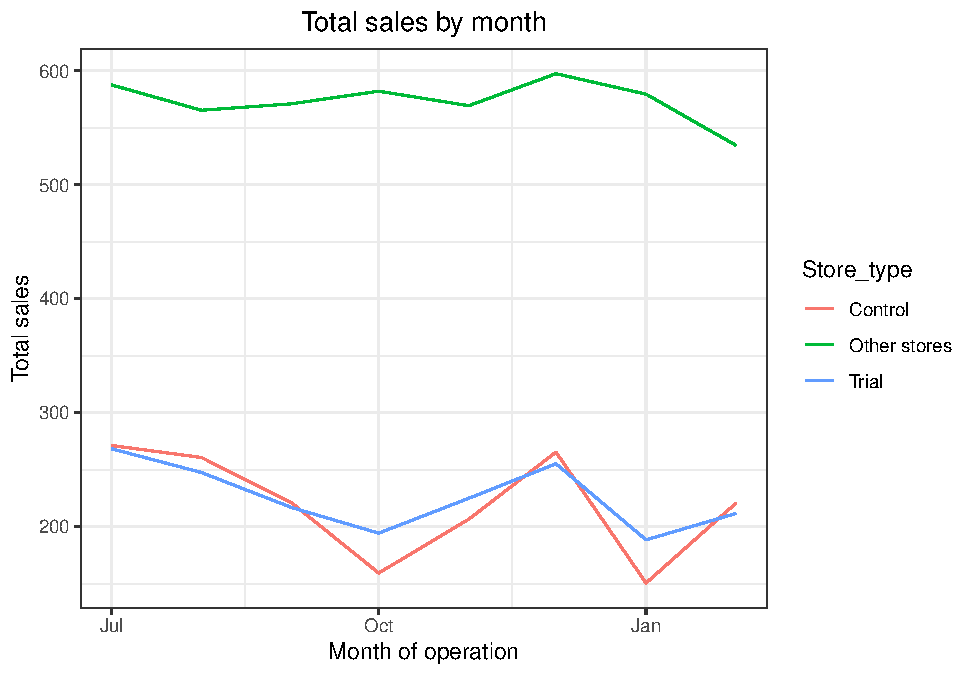
\includegraphics{InsideSherpa_Task2_files/figure-latex/unnamed-chunk-7-1.pdf}
Next, number of customers.

\begin{Shaded}
\begin{Highlighting}[]
\DocumentationTok{\#\#\#\# Conduct visual checks on customer count trends by comparing the trial store }
\DocumentationTok{\#\#\#\# to the control store and other stores.}
\NormalTok{measureOverTimeCusts }\OtherTok{\textless{}{-}}\NormalTok{ measureOverTime}
\NormalTok{pastCustomers }\OtherTok{\textless{}{-}}\NormalTok{ measureOverTimeCusts[, Store\_type }\SpecialCharTok{:=} \FunctionTok{ifelse}\NormalTok{(STORE\_NBR }\SpecialCharTok{==}\NormalTok{ trial\_store, }\StringTok{"Trial"}\NormalTok{,}
                                      \FunctionTok{ifelse}\NormalTok{(STORE\_NBR }\SpecialCharTok{==}\NormalTok{ control\_store, }\StringTok{"Control"}\NormalTok{, }\StringTok{"Other stores"}\NormalTok{))}
\NormalTok{][, numberCustomers }\SpecialCharTok{:=} \FunctionTok{mean}\NormalTok{(nCustomers), by }\OtherTok{=} \FunctionTok{c}\NormalTok{(}\StringTok{"YEARMONTH"}\NormalTok{, }\StringTok{"Store\_type"}\NormalTok{)}
\NormalTok{][, TransactionMonth }\SpecialCharTok{:=} \FunctionTok{as.Date}\NormalTok{(}\FunctionTok{paste}\NormalTok{(YEARMONTH }\SpecialCharTok{\%/\%} \DecValTok{100}\NormalTok{, YEARMONTH }\SpecialCharTok{\%\%} \DecValTok{100}\NormalTok{, }\DecValTok{1}\NormalTok{, }\AttributeTok{sep =} \StringTok{"{-}"}\NormalTok{), }\StringTok{"\%Y{-}\%m{-}\%d"}\NormalTok{)}
\NormalTok{][YEARMONTH }\SpecialCharTok{\textless{}} \DecValTok{201903}\NormalTok{ , ]}
\FunctionTok{ggplot}\NormalTok{(pastCustomers, }\FunctionTok{aes}\NormalTok{(TransactionMonth, numberCustomers, }\AttributeTok{color =}\NormalTok{ Store\_type)) }\SpecialCharTok{+}
  \FunctionTok{geom\_line}\NormalTok{() }\SpecialCharTok{+}
  \FunctionTok{labs}\NormalTok{(}\AttributeTok{x =} \StringTok{"Month of operation"}\NormalTok{, }\AttributeTok{y =} \StringTok{"Total number of customers"}\NormalTok{, }\AttributeTok{title =} \StringTok{"Total number of customers by month"}\NormalTok{)}
\end{Highlighting}
\end{Shaded}

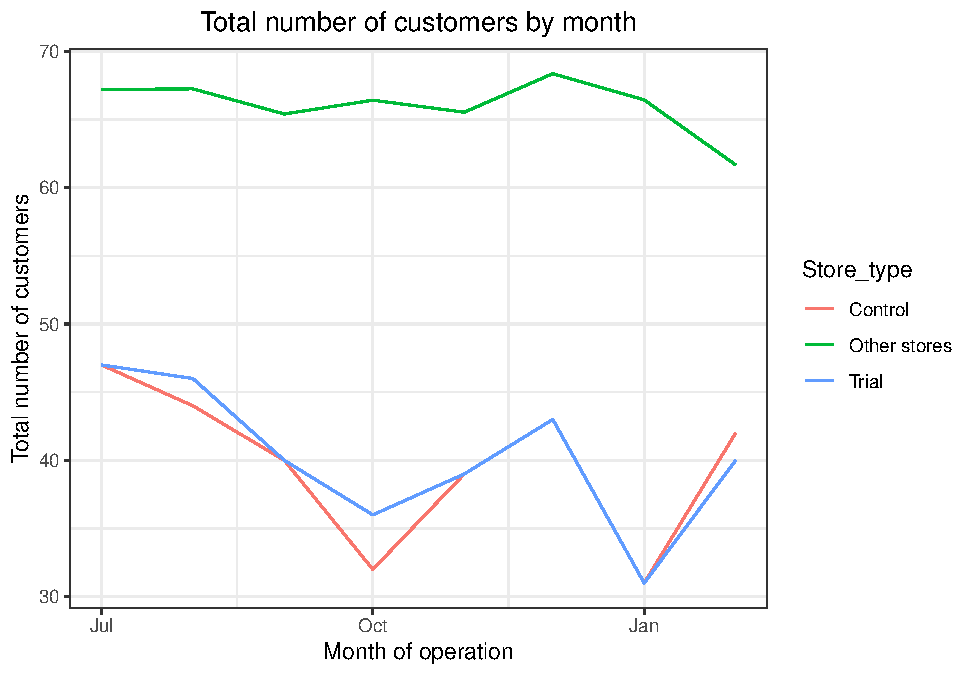
\includegraphics{InsideSherpa_Task2_files/figure-latex/unnamed-chunk-8-1.pdf}
\#\# Assessment of trial The trial period goes from the start of
February 2019 to April 2019. We now want to see if there has been an
uplift in overall chip sales. We'll start with scaling the control
store's sales to a level similar to control for any differences between
the two stores outside of the trial period.

\begin{Shaded}
\begin{Highlighting}[]
\DocumentationTok{\#\#\#\# Scale pre{-}trial control sales to match pre{-}trial trial store sales}
\NormalTok{scalingFactorForControlSales }\OtherTok{\textless{}{-}}\NormalTok{ preTrialMeasures[STORE\_NBR }\SpecialCharTok{==}\NormalTok{ trial\_store }\SpecialCharTok{\&}
\NormalTok{YEARMONTH }\SpecialCharTok{\textless{}} \DecValTok{201902}\NormalTok{, }\FunctionTok{sum}\NormalTok{(totSales)]}\SpecialCharTok{/}\NormalTok{preTrialMeasures[STORE\_NBR }\SpecialCharTok{==}\NormalTok{ control\_store }\SpecialCharTok{\&}
\NormalTok{YEARMONTH }\SpecialCharTok{\textless{}} \DecValTok{201902}\NormalTok{, }\FunctionTok{sum}\NormalTok{(totSales)]}
\DocumentationTok{\#\#\#\# Apply the scaling factor}
\NormalTok{measureOverTimeSales }\OtherTok{\textless{}{-}}\NormalTok{ measureOverTime}
\NormalTok{scaledControlSales }\OtherTok{\textless{}{-}}\NormalTok{ measureOverTimeSales[STORE\_NBR }\SpecialCharTok{==}\NormalTok{ control\_store, ][ ,}
\NormalTok{controlSales }\SpecialCharTok{:=}\NormalTok{ totSales }\SpecialCharTok{*}\NormalTok{ scalingFactorForControlSales]}
\end{Highlighting}
\end{Shaded}

Now that we have comparable sales figures for the control store, we can
calculate the percentage difference between the scaled control sales and
the trial store's sales during the trial period.

\begin{Shaded}
\begin{Highlighting}[]
\DocumentationTok{\#\#\#\# Calculate the percentage difference between scaled control sales and trial sales}
\NormalTok{percentageDiff }\OtherTok{\textless{}{-}} \FunctionTok{merge}\NormalTok{(scaledControlSales[, }\FunctionTok{c}\NormalTok{(}\StringTok{"YEARMONTH"}\NormalTok{, }\StringTok{"controlSales"}\NormalTok{)],}
\NormalTok{                        measureOverTime[STORE\_NBR }\SpecialCharTok{==}\NormalTok{ trial\_store, }\FunctionTok{c}\NormalTok{(}\StringTok{"totSales"}\NormalTok{, }\StringTok{"YEARMONTH"}\NormalTok{)],}
                        \AttributeTok{by =} \StringTok{"YEARMONTH"}\NormalTok{)[, percentageDiff }\SpecialCharTok{:=} \FunctionTok{abs}\NormalTok{(controlSales}\SpecialCharTok{{-}}\NormalTok{totSales)}\SpecialCharTok{/}\NormalTok{controlSales]}
\end{Highlighting}
\end{Shaded}

\begin{Shaded}
\begin{Highlighting}[]
\NormalTok{percentageDiff }\CommentTok{\# between control store sales and trial store sales}
\end{Highlighting}
\end{Shaded}

Let's see if the difference is significant!

\begin{Shaded}
\begin{Highlighting}[]
\DocumentationTok{\#\#\#\# As our null hypothesis is that the trial period is the same as the pre{-}trial}
\DocumentationTok{\#\#\#\# period, let\textquotesingle{}s take the standard deviation based on the scaled percentage difference}
\DocumentationTok{\#\#\#\# in the pre{-}trial period}
\NormalTok{stdDev }\OtherTok{\textless{}{-}} \FunctionTok{sd}\NormalTok{(percentageDiff[YEARMONTH }\SpecialCharTok{\textless{}} \DecValTok{201902}\NormalTok{ , percentageDiff])}
\DocumentationTok{\#\#\#\# Note that there are 8 months in the pre{-}trial period}
\DocumentationTok{\#\#\#\# hence 8 {-} 1 = 7 degrees of freedom}
\NormalTok{degreesOfFreedom }\OtherTok{\textless{}{-}} \DecValTok{7}
\DocumentationTok{\#\#\#\# We will test with a null hypothesis of there being 0 difference between trial}
\DocumentationTok{\#\#\#\# and control stores.}
\DocumentationTok{\#\#\#\# Calculate the t{-}values for the trial months. After that, find the 95th percentile of the t distribution with the appropriate degrees of freedom}
\DocumentationTok{\#\#\#\# to check whether the hypothesis is statistically significant.}
\DocumentationTok{\#\#\#\# The test statistic here is (x {-} u)/standard deviation}
\NormalTok{percentageDiff[, tValue }\SpecialCharTok{:=}\NormalTok{ (percentageDiff }\SpecialCharTok{{-}} \DecValTok{0}\NormalTok{)}\SpecialCharTok{/}\NormalTok{stdDev}
\NormalTok{               ][, TransactionMonth }\SpecialCharTok{:=} \FunctionTok{as.Date}\NormalTok{(}\FunctionTok{paste}\NormalTok{(YEARMONTH }\SpecialCharTok{\%/\%} \DecValTok{100}\NormalTok{, YEARMONTH }\SpecialCharTok{\%\%} \DecValTok{100}\NormalTok{, }\DecValTok{1}\NormalTok{, }
                                                     \AttributeTok{sep =} \StringTok{"{-}"}\NormalTok{), }\StringTok{"\%Y{-}\%m{-}\%d"}\NormalTok{)}
\NormalTok{][YEARMONTH }\SpecialCharTok{\textless{}} \DecValTok{201905} \SpecialCharTok{\&}\NormalTok{ YEARMONTH }\SpecialCharTok{\textgreater{}} \DecValTok{201901}\NormalTok{, .(TransactionMonth,tValue)]}
\end{Highlighting}
\end{Shaded}

\begin{verbatim}
##    TransactionMonth    tValue
##              <Date>     <num>
## 1:       2019-02-01  1.223912
## 2:       2019-03-01  5.633494
## 3:       2019-04-01 11.336505
\end{verbatim}

\begin{Shaded}
\begin{Highlighting}[]
\DocumentationTok{\#\#\#\# Find the 95th percentile of the t distribution with the appropriate}
\DocumentationTok{\#\#\#\# degrees of freedom to compare against}
\FunctionTok{qt}\NormalTok{(}\FloatTok{0.95}\NormalTok{, }\AttributeTok{df =}\NormalTok{ degreesOfFreedom)}
\end{Highlighting}
\end{Shaded}

\begin{verbatim}
## [1] 1.894579
\end{verbatim}

We can observe that the t-value is much larger than the 95th percentile
value of the t-distribution for March and April - i.e.~the increase in
sales in the trial store in March and April is statistically greater
than in the control store. Let's create a more visual version of this by
plotting the sales of the control store, the sales of the trial stores
and the 95th percentile value of sales of the control store.

\begin{Shaded}
\begin{Highlighting}[]
\NormalTok{measureOverTimeSales }\OtherTok{\textless{}{-}}\NormalTok{ measureOverTime}

\DocumentationTok{\#\#\#\# Trial and control store total sales}
\DocumentationTok{\#\#\#\# Create new variables Store\_type, totSales and TransactionMonth in the data table.}
\NormalTok{pastSales }\OtherTok{\textless{}{-}}\NormalTok{ measureOverTimeSales[, Store\_type }\SpecialCharTok{:=} \FunctionTok{ifelse}\NormalTok{(STORE\_NBR }\SpecialCharTok{==}\NormalTok{ trial\_store, }\StringTok{"Trial"}\NormalTok{,}
\FunctionTok{ifelse}\NormalTok{(STORE\_NBR }\SpecialCharTok{==}\NormalTok{ control\_store, }\StringTok{"Control"}\NormalTok{, }\StringTok{"Other stores"}\NormalTok{))}
\NormalTok{][, totSales }\SpecialCharTok{:=} \FunctionTok{mean}\NormalTok{(totSales), by }\OtherTok{=} \FunctionTok{c}\NormalTok{(}\StringTok{"YEARMONTH"}\NormalTok{, }\StringTok{"Store\_type"}\NormalTok{)}
\NormalTok{][, TransactionMonth }\SpecialCharTok{:=} \FunctionTok{as.Date}\NormalTok{(}\FunctionTok{paste}\NormalTok{(YEARMONTH }\SpecialCharTok{\%/\%} \DecValTok{100}\NormalTok{, YEARMONTH }\SpecialCharTok{\%\%} \DecValTok{100}\NormalTok{, }\DecValTok{1}\NormalTok{, }\AttributeTok{sep =} \StringTok{"{-}"}\NormalTok{), }\StringTok{"\%Y{-}\%m{-}\%d"}\NormalTok{)}
\NormalTok{][Store\_type }\SpecialCharTok{\%in\%} \FunctionTok{c}\NormalTok{(}\StringTok{"Trial"}\NormalTok{, }\StringTok{"Control"}\NormalTok{), ]}

\DocumentationTok{\#\#\#\# Control store 95th percentile}
\NormalTok{pastSales\_Controls95 }\OtherTok{\textless{}{-}}\NormalTok{ pastSales[Store\_type }\SpecialCharTok{==} \StringTok{"Control"}\NormalTok{,}
\NormalTok{ ][, totSales }\SpecialCharTok{:=}\NormalTok{ totSales }\SpecialCharTok{*}\NormalTok{ (}\DecValTok{1} \SpecialCharTok{+}\NormalTok{ stdDev }\SpecialCharTok{*} \DecValTok{2}\NormalTok{)}
\NormalTok{ ][, Store\_type }\SpecialCharTok{:=} \StringTok{"Control 95th \% confidence}
\StringTok{interval"}\NormalTok{]}

\DocumentationTok{\#\#\#\# Control store 5th percentile}
\NormalTok{pastSales\_Controls5 }\OtherTok{\textless{}{-}}\NormalTok{ pastSales[Store\_type }\SpecialCharTok{==} \StringTok{"Control"}\NormalTok{,}
\NormalTok{ ][, totSales }\SpecialCharTok{:=}\NormalTok{ totSales }\SpecialCharTok{*}\NormalTok{ (}\DecValTok{1} \SpecialCharTok{{-}}\NormalTok{ stdDev }\SpecialCharTok{*} \DecValTok{2}\NormalTok{)}
\NormalTok{ ][, Store\_type }\SpecialCharTok{:=} \StringTok{"Control 5th \% confidence}
\StringTok{interval"}\NormalTok{]}
\NormalTok{trialAssessment }\OtherTok{\textless{}{-}} \FunctionTok{rbind}\NormalTok{(pastSales, pastSales\_Controls95, pastSales\_Controls5)}

\DocumentationTok{\#\#\#\# Plotting these in one nice graph}
\FunctionTok{ggplot}\NormalTok{(trialAssessment, }\FunctionTok{aes}\NormalTok{(TransactionMonth, totSales, }\AttributeTok{color =}\NormalTok{ Store\_type)) }\SpecialCharTok{+}
  \FunctionTok{geom\_rect}\NormalTok{(}\AttributeTok{data =}\NormalTok{ trialAssessment[ YEARMONTH }\SpecialCharTok{\textless{}} \DecValTok{201905} \SpecialCharTok{\&}\NormalTok{ YEARMONTH }\SpecialCharTok{\textgreater{}} \DecValTok{201901}\NormalTok{ ,],}
\FunctionTok{aes}\NormalTok{(}\AttributeTok{xmin =} \FunctionTok{min}\NormalTok{(TransactionMonth), }\AttributeTok{xmax =} \FunctionTok{max}\NormalTok{(TransactionMonth), }\AttributeTok{ymin =} \DecValTok{0}\NormalTok{ , }\AttributeTok{ymax =}
\ConstantTok{Inf}\NormalTok{, }\AttributeTok{color =} \ConstantTok{NULL}\NormalTok{), }\AttributeTok{show.legend =} \ConstantTok{FALSE}\NormalTok{) }\SpecialCharTok{+}
  \FunctionTok{geom\_line}\NormalTok{() }\SpecialCharTok{+}
  \FunctionTok{labs}\NormalTok{(}\AttributeTok{x =} \StringTok{"Month of operation"}\NormalTok{, }\AttributeTok{y =} \StringTok{"Total sales"}\NormalTok{, }\AttributeTok{title =} \StringTok{"Total sales by month"}\NormalTok{)}
\end{Highlighting}
\end{Shaded}

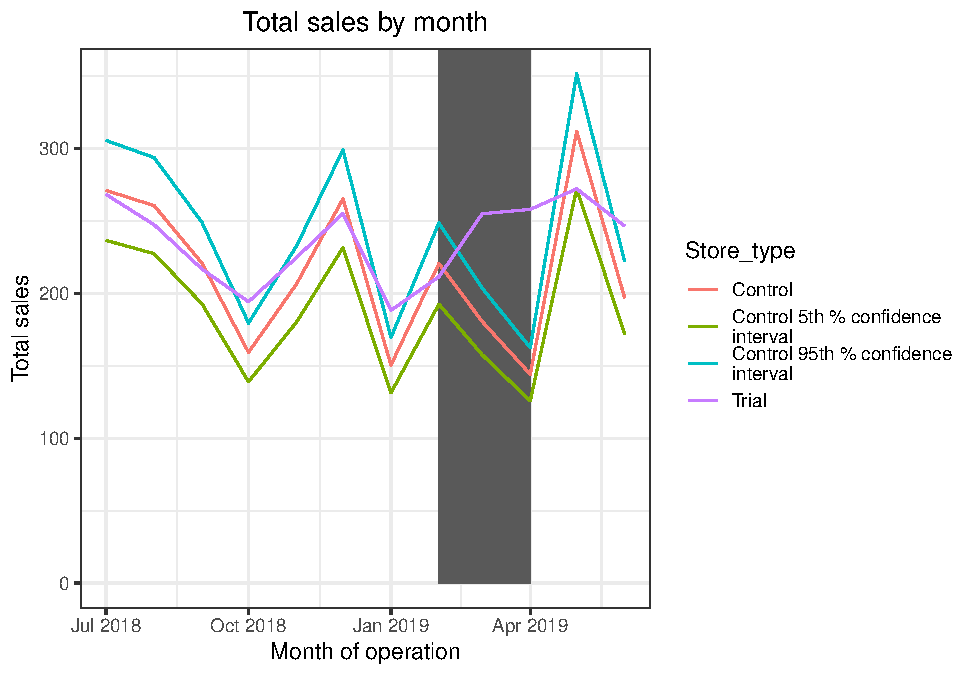
\includegraphics{InsideSherpa_Task2_files/figure-latex/unnamed-chunk-13-1}
The results show that the trial in store 77 is significantly different
to its control store in the trial period as the trial store performance
lies outside the 5\% to 95\% confidence interval of the control store in
two of the three trial months. Let's have a look at assessing this for
number of customers as well.

\begin{Shaded}
\begin{Highlighting}[]
\DocumentationTok{\#\#\#\# This would be a repeat of the steps before for total sales}
\DocumentationTok{\#\#\#\# Scale pre{-}trial control customers to match pre{-}trial trial store customers}
\DocumentationTok{\#\#\#\# Compute a scaling factor to align control store customer counts to our trial store.}
\DocumentationTok{\#\#\#\# Then, apply the scaling factor to control store customer counts.}
\DocumentationTok{\#\#\#\# Finally, calculate the percentage difference between scaled control store customers and trial customers.}
\NormalTok{scalingFactorForControlCust }\OtherTok{\textless{}{-}}\NormalTok{ preTrialMeasures[STORE\_NBR }\SpecialCharTok{==}\NormalTok{ trial\_store }\SpecialCharTok{\&}
\NormalTok{YEARMONTH }\SpecialCharTok{\textless{}} \DecValTok{201902}\NormalTok{, }\FunctionTok{sum}\NormalTok{(nCustomers)] }\SpecialCharTok{/}\NormalTok{ preTrialMeasures[STORE\_NBR }\SpecialCharTok{==}
\NormalTok{control\_store }\SpecialCharTok{\&}\NormalTok{ YEARMONTH }\SpecialCharTok{\textless{}} \DecValTok{201902}\NormalTok{, }\FunctionTok{sum}\NormalTok{(nCustomers)]}
\NormalTok{measureOverTimeCusts }\OtherTok{\textless{}{-}}\NormalTok{ measureOverTime}
\NormalTok{scaledControlCustomers }\OtherTok{\textless{}{-}}\NormalTok{ measureOverTimeCusts[STORE\_NBR }\SpecialCharTok{==}\NormalTok{ control\_store,}
\NormalTok{][ , controlCustomers }\SpecialCharTok{:=}\NormalTok{ nCustomers }\SpecialCharTok{*}\NormalTok{ scalingFactorForControlCust}
\NormalTok{][, Store\_type }\SpecialCharTok{:=} \FunctionTok{ifelse}\NormalTok{(STORE\_NBR }\SpecialCharTok{==}\NormalTok{trial\_store, }\StringTok{"Trial"}\NormalTok{,}
\FunctionTok{ifelse}\NormalTok{(STORE\_NBR }\SpecialCharTok{==}\NormalTok{ control\_store,}\StringTok{"Control"}\NormalTok{, }\StringTok{"Other stores"}\NormalTok{))]}
\NormalTok{percentageDiff }\OtherTok{\textless{}{-}} \FunctionTok{merge}\NormalTok{(scaledControlCustomers[, }\FunctionTok{c}\NormalTok{(}\StringTok{"YEARMONTH"}\NormalTok{, }\StringTok{"controlCustomers"}\NormalTok{)],}
\NormalTok{measureOverTimeCusts[STORE\_NBR }\SpecialCharTok{==}\NormalTok{ trial\_store,}\FunctionTok{c}\NormalTok{(}\StringTok{"nCustomers"}\NormalTok{, }\StringTok{"YEARMONTH"}\NormalTok{)],}
\AttributeTok{by =} \StringTok{"YEARMONTH"}
\NormalTok{)[, percentageDiff }\SpecialCharTok{:=} \FunctionTok{abs}\NormalTok{(controlCustomers}\SpecialCharTok{{-}}\NormalTok{nCustomers)}\SpecialCharTok{/}\NormalTok{controlCustomers]}
\end{Highlighting}
\end{Shaded}

Let's again see if the difference is significant visually!

\begin{Shaded}
\begin{Highlighting}[]
\DocumentationTok{\#\#\#\# As our null hypothesis is that the trial period is the same as the pre{-}trial }
\DocumentationTok{\#\#\#\# period, let\textquotesingle{}s take the standard deviation based on the scaled percentage difference}
\DocumentationTok{\#\#\#\# in the pre{-}trial period}
\NormalTok{stdDev }\OtherTok{\textless{}{-}} \FunctionTok{sd}\NormalTok{(percentageDiff[YEARMONTH }\SpecialCharTok{\textless{}} \DecValTok{201902}\NormalTok{ , percentageDiff])}
\NormalTok{degreesOfFreedom }\OtherTok{\textless{}{-}} \DecValTok{7}
\DocumentationTok{\#\#\#\# Trial and control store number of customers}
\NormalTok{pastCustomers }\OtherTok{\textless{}{-}}\NormalTok{ measureOverTimeCusts[, nCusts }\SpecialCharTok{:=} \FunctionTok{mean}\NormalTok{(nCustomers), by }\OtherTok{=}
\FunctionTok{c}\NormalTok{(}\StringTok{"YEARMONTH"}\NormalTok{, }\StringTok{"Store\_type"}\NormalTok{)}
\NormalTok{                            ][Store\_type }\SpecialCharTok{\%in\%} \FunctionTok{c}\NormalTok{(}\StringTok{"Trial"}\NormalTok{, }\StringTok{"Control"}\NormalTok{), ]}
\DocumentationTok{\#\#\#\# Control store 95th percentile}
\NormalTok{pastCustomers\_Controls95 }\OtherTok{\textless{}{-}}\NormalTok{ pastCustomers[Store\_type }\SpecialCharTok{==} \StringTok{"Control"}\NormalTok{,}
\NormalTok{                                ][, nCusts }\SpecialCharTok{:=}\NormalTok{ nCusts }\SpecialCharTok{*}\NormalTok{ (}\DecValTok{1} \SpecialCharTok{+}\NormalTok{ stdDev }\SpecialCharTok{*} \DecValTok{2}\NormalTok{)}
\NormalTok{                                ][, Store\_type }\SpecialCharTok{:=} \StringTok{"Control 95th \% confidence}
\StringTok{interval"}\NormalTok{]}
\DocumentationTok{\#\#\#\# Control store 5th percentile}
\NormalTok{pastCustomers\_Controls5 }\OtherTok{\textless{}{-}}\NormalTok{ pastCustomers[Store\_type }\SpecialCharTok{==} \StringTok{"Control"}\NormalTok{,}
\NormalTok{                                ][, nCusts }\SpecialCharTok{:=}\NormalTok{ nCusts }\SpecialCharTok{*}\NormalTok{ (}\DecValTok{1} \SpecialCharTok{{-}}\NormalTok{ stdDev }\SpecialCharTok{*} \DecValTok{2}\NormalTok{)}
\NormalTok{                                ][, Store\_type }\SpecialCharTok{:=} \StringTok{"Control 5th \% confidence}
\StringTok{interval"}\NormalTok{]}
\NormalTok{trialAssessment }\OtherTok{\textless{}{-}} \FunctionTok{rbind}\NormalTok{(pastCustomers, pastCustomers\_Controls95,}
\NormalTok{pastCustomers\_Controls5)}
\DocumentationTok{\#\#\#\# Plot everything into one nice graph.}
\DocumentationTok{\#\#\#\# geom\_rect creates a rectangle in the plot. Use this to highlight the}
\DocumentationTok{\#\#\#\# trial period in our graph.}
\FunctionTok{ggplot}\NormalTok{(trialAssessment, }\FunctionTok{aes}\NormalTok{(TransactionMonth, nCusts, }\AttributeTok{color =}\NormalTok{ Store\_type)) }\SpecialCharTok{+} 
  \FunctionTok{geom\_rect}\NormalTok{(}\AttributeTok{data =}\NormalTok{ trialAssessment[ YEARMONTH }\SpecialCharTok{\textless{}} \DecValTok{201905} \SpecialCharTok{\&}\NormalTok{ YEARMONTH }\SpecialCharTok{\textgreater{}} \DecValTok{201901}\NormalTok{ ,],}
\FunctionTok{aes}\NormalTok{(}\AttributeTok{xmin =} \FunctionTok{min}\NormalTok{(TransactionMonth), }\AttributeTok{xmax =} \FunctionTok{max}\NormalTok{(TransactionMonth), }\AttributeTok{ymin =} \DecValTok{0}\NormalTok{ ,}
\AttributeTok{ymax =} \ConstantTok{Inf}\NormalTok{, }\AttributeTok{color =} \ConstantTok{NULL}\NormalTok{), }\AttributeTok{show.legend =} \ConstantTok{FALSE}\NormalTok{) }\SpecialCharTok{+} 
  \FunctionTok{geom\_line}\NormalTok{() }\SpecialCharTok{+} \FunctionTok{labs}\NormalTok{(}\AttributeTok{x =} \StringTok{"Month of operation"}\NormalTok{, }\AttributeTok{y =} \StringTok{"Total number of customers"}\NormalTok{, }\AttributeTok{title =} \StringTok{"Total number of customers by month"}\NormalTok{)}
\end{Highlighting}
\end{Shaded}

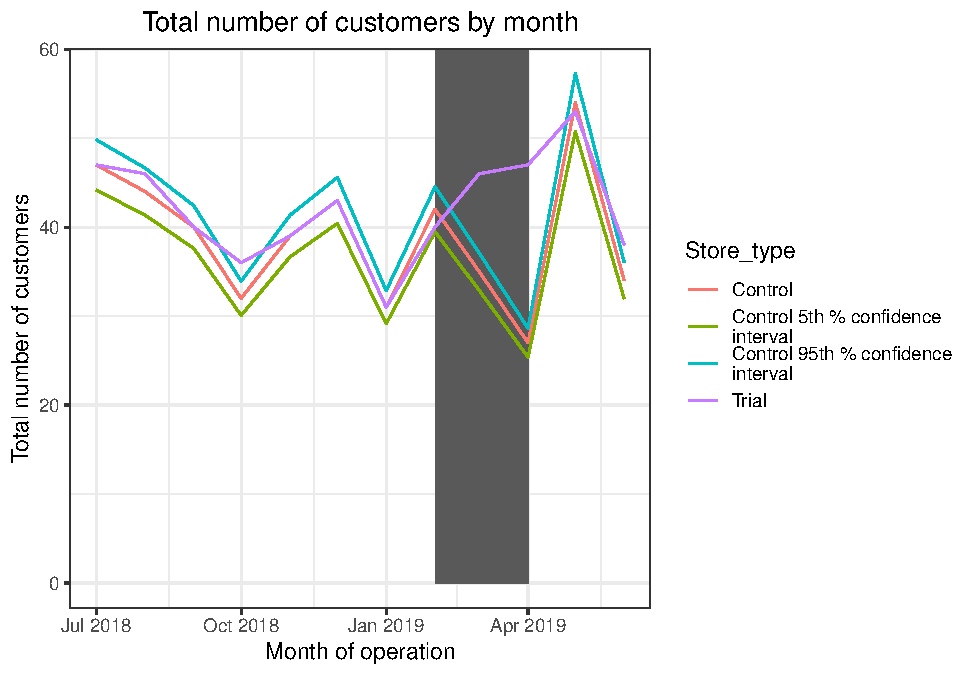
\includegraphics{InsideSherpa_Task2_files/figure-latex/unnamed-chunk-15-1}
Let's repeat finding the control store and assessing the impact of the
trial for each of the other two trial stores. \#\# Trial store 86

\begin{Shaded}
\begin{Highlighting}[]
\DocumentationTok{\#\#\#\# Calculate the metrics below as we did for the first trial store.}
\NormalTok{measureOverTime }\OtherTok{\textless{}{-}}\NormalTok{ data[, .(}\AttributeTok{totSales =} \FunctionTok{sum}\NormalTok{(TOT\_SALES),}
                            \AttributeTok{nCustomers =} \FunctionTok{uniqueN}\NormalTok{(LYLTY\_CARD\_NBR),}
                            \AttributeTok{nTxnPerCust =}\NormalTok{ (}\FunctionTok{uniqueN}\NormalTok{(TXN\_ID))}\SpecialCharTok{/}\NormalTok{(}\FunctionTok{uniqueN}\NormalTok{(LYLTY\_CARD\_NBR)),}
                            \AttributeTok{nChipsPerTxn =}\NormalTok{ (}\FunctionTok{sum}\NormalTok{(PROD\_QTY))}\SpecialCharTok{/}\NormalTok{(}\FunctionTok{uniqueN}\NormalTok{(TXN\_ID)) , }
                            \AttributeTok{avgPricePerUnit =} \FunctionTok{sum}\NormalTok{(TOT\_SALES)}\SpecialCharTok{/}\FunctionTok{sum}\NormalTok{(PROD\_QTY) ) , by }\OtherTok{=} \FunctionTok{c}\NormalTok{(}\StringTok{"STORE\_NBR"}\NormalTok{, }\StringTok{"YEARMONTH"}\NormalTok{)][}\FunctionTok{order}\NormalTok{(STORE\_NBR, YEARMONTH)]}

\DocumentationTok{\#\#\#\# Use the functions we created earlier to calculate correlations and magnitude for each potential control store}
\NormalTok{trial\_store }\OtherTok{\textless{}{-}} \DecValTok{86}
\NormalTok{corr\_nSales }\OtherTok{\textless{}{-}} \FunctionTok{calculateCorrelation}\NormalTok{(preTrialMeasures, }\FunctionTok{quote}\NormalTok{(totSales),trial\_store)}
\NormalTok{corr\_nCustomers }\OtherTok{\textless{}{-}} \FunctionTok{calculateCorrelation}\NormalTok{(preTrialMeasures, }\FunctionTok{quote}\NormalTok{(nCustomers), trial\_store)}
\NormalTok{magnitude\_nSales }\OtherTok{\textless{}{-}} \FunctionTok{calculateMagnitudeDistance}\NormalTok{(preTrialMeasures, }\FunctionTok{quote}\NormalTok{(totSales), trial\_store)}
\NormalTok{magnitude\_nCustomers }\OtherTok{\textless{}{-}} \FunctionTok{calculateMagnitudeDistance}\NormalTok{(preTrialMeasures, }\FunctionTok{quote}\NormalTok{(nCustomers), trial\_store)}
\DocumentationTok{\#\#\#\# Now, create a combined score composed of correlation and magnitude}
\NormalTok{corr\_weight }\OtherTok{\textless{}{-}} \FloatTok{0.5}
\NormalTok{score\_nSales }\OtherTok{\textless{}{-}} \FunctionTok{merge}\NormalTok{(corr\_nSales, magnitude\_nSales, }\AttributeTok{by =} \FunctionTok{c}\NormalTok{(}\StringTok{"Store1"}\NormalTok{, }\StringTok{"Store2"}\NormalTok{))[ , scoreNSales }\SpecialCharTok{:=}\NormalTok{ (corr\_measure }\SpecialCharTok{+}\NormalTok{ mag\_measure)}\SpecialCharTok{/}\DecValTok{2}\NormalTok{]}
\NormalTok{score\_nCustomers }\OtherTok{\textless{}{-}} \FunctionTok{merge}\NormalTok{(corr\_nCustomers, magnitude\_nCustomers, }\AttributeTok{by =} \FunctionTok{c}\NormalTok{(}\StringTok{"Store1"}\NormalTok{, }\StringTok{"Store2"}\NormalTok{))[ , scoreNCust }\SpecialCharTok{:=}\NormalTok{ (corr\_measure }\SpecialCharTok{+}\NormalTok{ mag\_measure)}\SpecialCharTok{/}\DecValTok{2}\NormalTok{]}

\DocumentationTok{\#\#\#\# Finally, combine scores across the drivers using a simple average.}
\NormalTok{score\_Control }\OtherTok{\textless{}{-}} \FunctionTok{merge}\NormalTok{(score\_nSales, score\_nCustomers, }\AttributeTok{by =} \FunctionTok{c}\NormalTok{(}\StringTok{"Store1"}\NormalTok{,}\StringTok{"Store2"}\NormalTok{))}
\NormalTok{score\_Control[, finalControlScore }\SpecialCharTok{:=}\NormalTok{ scoreNSales }\SpecialCharTok{*} \FloatTok{0.5} \SpecialCharTok{+}\NormalTok{ scoreNCust }\SpecialCharTok{*} \FloatTok{0.5}\NormalTok{]}
\DocumentationTok{\#\#\#\# Select control stores based on the highest matching store}
\DocumentationTok{\#\#\#\# (closest to 1 but not the store itself, i.e. the second ranked highest store)}
\DocumentationTok{\#\#\#\# Select control store for trial store 86}
\NormalTok{control\_store }\OtherTok{\textless{}{-}}\NormalTok{ score\_Control[Store1 }\SpecialCharTok{==}\NormalTok{ trial\_store,}
\NormalTok{][}\FunctionTok{order}\NormalTok{(}\SpecialCharTok{{-}}\NormalTok{finalControlScore)][}\DecValTok{2}\NormalTok{, Store2]}
\NormalTok{control\_store}
\end{Highlighting}
\end{Shaded}

\begin{verbatim}
## [1] 155
\end{verbatim}

Looks like store 155 will be a control store for trial store 86. Again,
let's check visually if the drivers are indeed similar in the period
before the trial. We'll look at total sales first.

\begin{Shaded}
\begin{Highlighting}[]
\DocumentationTok{\#\#\#\# Conduct visual checks on trends based on the drivers}
\NormalTok{measureOverTimeSales }\OtherTok{\textless{}{-}}\NormalTok{ measureOverTime}
\NormalTok{pastSales }\OtherTok{\textless{}{-}}\NormalTok{ measureOverTimeSales[, Store\_type}\SpecialCharTok{:=} \FunctionTok{ifelse}\NormalTok{(STORE\_NBR }\SpecialCharTok{==}\NormalTok{ trial\_store, }\StringTok{"Trial"}\NormalTok{, }\FunctionTok{ifelse}\NormalTok{(STORE\_NBR}\SpecialCharTok{==}\NormalTok{ control\_store, }\StringTok{"Control"}\NormalTok{, }\StringTok{"Other stores"}\NormalTok{))][, totSales }\SpecialCharTok{:=} \FunctionTok{mean}\NormalTok{(totSales), by }\OtherTok{=} \FunctionTok{c}\NormalTok{(}\StringTok{"YEARMONTH"}\NormalTok{, }\StringTok{"Store\_type"}\NormalTok{)][, TransactionMonth}\SpecialCharTok{:=} \FunctionTok{as.Date}\NormalTok{(}\FunctionTok{paste}\NormalTok{(YEARMONTH}\SpecialCharTok{\%/\%}\DecValTok{100}\NormalTok{, YEARMONTH}\SpecialCharTok{\%\%} \DecValTok{100}\NormalTok{, }\DecValTok{1}\NormalTok{, }\AttributeTok{sep =} \StringTok{"{-}"}\NormalTok{), }\StringTok{"\%Y{-}\%m{-}\%d"}\NormalTok{)][YEARMONTH }\SpecialCharTok{\textless{}}\DecValTok{210903}\NormalTok{] }

\FunctionTok{ggplot}\NormalTok{(pastSales, }\FunctionTok{aes}\NormalTok{(TransactionMonth, totSales, }\AttributeTok{color =}\NormalTok{ Store\_type)) }\SpecialCharTok{+}
  \FunctionTok{geom\_line}\NormalTok{(}\FunctionTok{aes}\NormalTok{(}\AttributeTok{linetype =}\NormalTok{ Store\_type)) }\SpecialCharTok{+}
  \FunctionTok{labs}\NormalTok{(}\AttributeTok{x =} \StringTok{"Month of operation"}\NormalTok{, }\AttributeTok{y =} \StringTok{"Total sales"}\NormalTok{, }\AttributeTok{title =} \StringTok{"Total sales by month"}\NormalTok{)}
\end{Highlighting}
\end{Shaded}

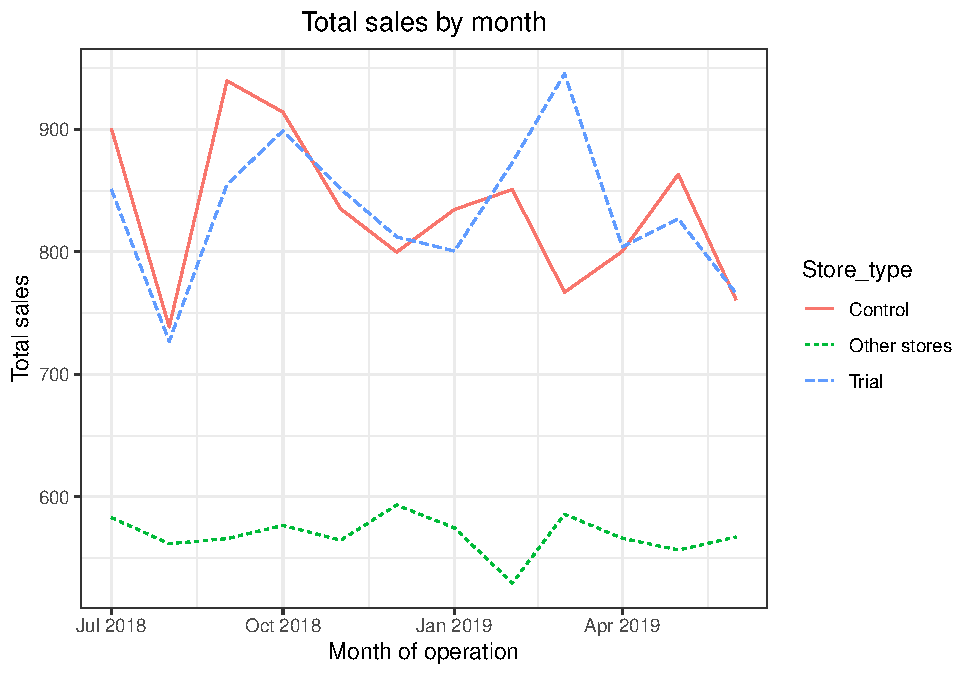
\includegraphics{InsideSherpa_Task2_files/figure-latex/unnamed-chunk-17-1.pdf}
Great, sales are trending in a similar way. Next, number of customers.

\begin{Shaded}
\begin{Highlighting}[]
\DocumentationTok{\#\#\#\# Conduct visual checks on trends based on the drivers}
\NormalTok{measureOverTimeCusts }\OtherTok{\textless{}{-}}\NormalTok{ measureOverTime}
\NormalTok{pastCustomers }\OtherTok{\textless{}{-}}\NormalTok{ measureOverTimeCusts[, Store\_type }\SpecialCharTok{:=} \FunctionTok{ifelse}\NormalTok{(STORE\_NBR }\SpecialCharTok{==}\NormalTok{ trial\_store, }\StringTok{"Trial"}\NormalTok{,}
\FunctionTok{ifelse}\NormalTok{(STORE\_NBR }\SpecialCharTok{==}\NormalTok{ control\_store, }\StringTok{"Control"}\NormalTok{, }\StringTok{"Other stores"}\NormalTok{))}
\NormalTok{][, numberCustomers }\SpecialCharTok{:=} \FunctionTok{mean}\NormalTok{(nCustomers), by }\OtherTok{=} \FunctionTok{c}\NormalTok{(}\StringTok{"YEARMONTH"}\NormalTok{, }\StringTok{"Store\_type"}\NormalTok{)}
\NormalTok{][, TransactionMonth }\SpecialCharTok{:=} \FunctionTok{as.Date}\NormalTok{(}\FunctionTok{paste}\NormalTok{(YEARMONTH }\SpecialCharTok{\%/\%}
                                        \DecValTok{100}\NormalTok{, YEARMONTH }\SpecialCharTok{\%\%} \DecValTok{100}\NormalTok{, }\DecValTok{1}\NormalTok{, }\AttributeTok{sep =} \StringTok{"{-}"}\NormalTok{), }\StringTok{"\%Y{-}\%m{-}\%d"}\NormalTok{)}
\NormalTok{][YEARMONTH }\SpecialCharTok{\textless{}} \DecValTok{201903}\NormalTok{ , ]}

\FunctionTok{ggplot}\NormalTok{(pastCustomers, }\FunctionTok{aes}\NormalTok{(TransactionMonth, numberCustomers, }\AttributeTok{color =}\NormalTok{ Store\_type)) }\SpecialCharTok{+} 
  \FunctionTok{geom\_line}\NormalTok{() }\SpecialCharTok{+} 
  \FunctionTok{labs}\NormalTok{(}\AttributeTok{x =} \StringTok{"Month of operation"}\NormalTok{, }\AttributeTok{y =} \StringTok{"Total number of customers"}\NormalTok{, }\AttributeTok{title =} \StringTok{"Total number of customers by month"}\NormalTok{)}
\end{Highlighting}
\end{Shaded}

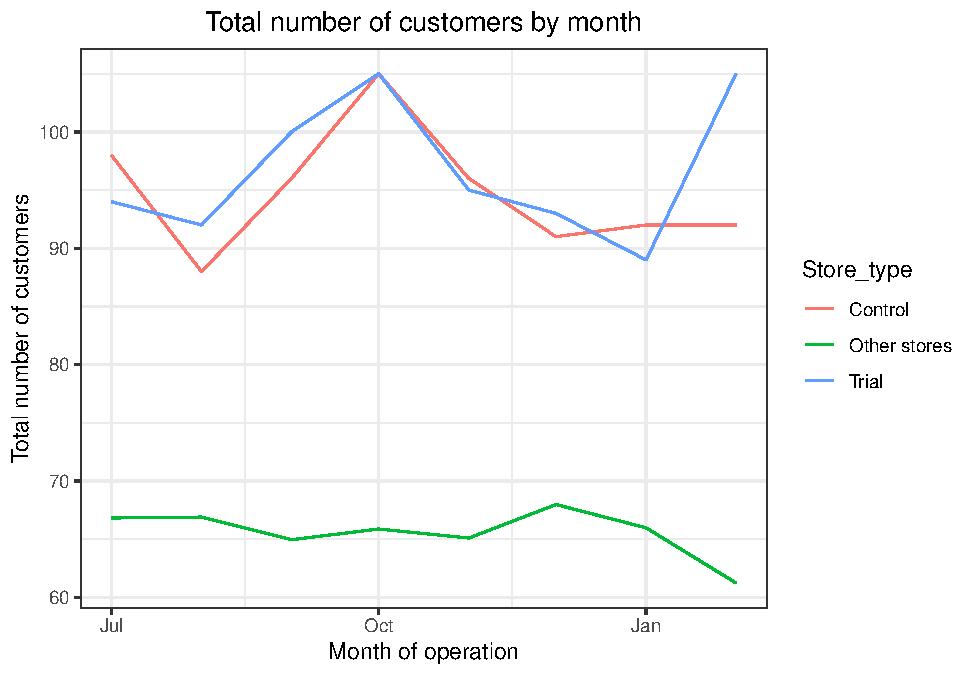
\includegraphics{InsideSherpa_Task2_files/figure-latex/unnamed-chunk-18-1.pdf}
Good, the trend in number of customers is also similar. Let's now assess
the impact of the trial on sales.

\begin{Shaded}
\begin{Highlighting}[]
\DocumentationTok{\#\#\#\# Scale pre{-}trial control sales to match pre{-}trial trial store sales}
\NormalTok{scalingFactorForControlSales }\OtherTok{\textless{}{-}}\NormalTok{ preTrialMeasures[STORE\_NBR }\SpecialCharTok{==}\NormalTok{ trial\_store }\SpecialCharTok{\&}
\NormalTok{YEARMONTH }\SpecialCharTok{\textless{}} \DecValTok{201902}\NormalTok{, }\FunctionTok{sum}\NormalTok{(totSales)]}\SpecialCharTok{/}\NormalTok{preTrialMeasures[STORE\_NBR }\SpecialCharTok{==}\NormalTok{ control\_store }\SpecialCharTok{\&}
\NormalTok{YEARMONTH }\SpecialCharTok{\textless{}} \DecValTok{201902}\NormalTok{, }\FunctionTok{sum}\NormalTok{(totSales)]}
\DocumentationTok{\#\#\#\# Apply the scaling factor}
\NormalTok{measureOverTimeSales }\OtherTok{\textless{}{-}}\NormalTok{ measureOverTime}
\NormalTok{scaledControlSales }\OtherTok{\textless{}{-}}\NormalTok{ measureOverTimeSales[STORE\_NBR }\SpecialCharTok{==}\NormalTok{ control\_store, ][ ,}
\NormalTok{controlSales }\SpecialCharTok{:=}\NormalTok{ totSales }\SpecialCharTok{*}\NormalTok{ scalingFactorForControlSales]}
\DocumentationTok{\#\#\#\# Calculate the percentage difference between scaled control sales and trial sales}
\DocumentationTok{\#\#\#\# When calculating percentage difference, remember to use absolute difference}
\NormalTok{percentageDiff }\OtherTok{\textless{}{-}} \FunctionTok{merge}\NormalTok{(scaledControlSales[, }\FunctionTok{c}\NormalTok{(}\StringTok{"YEARMONTH"}\NormalTok{, }\StringTok{"controlSales"}\NormalTok{)],}
\NormalTok{measureOverTime[STORE\_NBR }\SpecialCharTok{==}\NormalTok{ trial\_store, }\FunctionTok{c}\NormalTok{(}\StringTok{"totSales"}\NormalTok{, }\StringTok{"YEARMONTH"}\NormalTok{)],}
\AttributeTok{by =} \StringTok{"YEARMONTH"}
\NormalTok{)[, percentageDiff }\SpecialCharTok{:=} \FunctionTok{abs}\NormalTok{(controlSales}\SpecialCharTok{{-}}\NormalTok{totSales)}\SpecialCharTok{/}\NormalTok{controlSales]}

\DocumentationTok{\#\#\#\# As our null hypothesis is that the trial period is the same as the pre{-}trial}
\DocumentationTok{\#\#\#\# period, let\textquotesingle{}s take the standard deviation based on the scaled percentage difference}
\DocumentationTok{\#\#\#\# in the pre{-}trial period}
\DocumentationTok{\#\#\#\# Calculate the standard deviation of percentage differences during the pre{-}trial period}
\NormalTok{stdDev }\OtherTok{\textless{}{-}} \FunctionTok{sd}\NormalTok{(percentageDiff[YEARMONTH }\SpecialCharTok{\textless{}} \DecValTok{201902}\NormalTok{ , percentageDiff])}
\NormalTok{degreesOfFreedom }\OtherTok{\textless{}{-}} \DecValTok{7}

\DocumentationTok{\#\#\#\# Trial and control store total sales}
\DocumentationTok{\#\#\#\# Create a table with sales by store type and month.}
\DocumentationTok{\#\#\#\# We only need data for the trial and control store.}
\NormalTok{measureOverTimeSales }\OtherTok{\textless{}{-}}\NormalTok{ measureOverTime}
\NormalTok{pastSales }\OtherTok{\textless{}{-}}\NormalTok{ measureOverTimeSales[, Store\_type }\SpecialCharTok{:=} \FunctionTok{ifelse}\NormalTok{(STORE\_NBR }\SpecialCharTok{==}\NormalTok{ trial\_store, }\StringTok{"Trial"}\NormalTok{,}
\FunctionTok{ifelse}\NormalTok{(STORE\_NBR }\SpecialCharTok{==}\NormalTok{ control\_store, }\StringTok{"Control"}\NormalTok{, }\StringTok{"Other stores"}\NormalTok{))}
\NormalTok{][, totSales }\SpecialCharTok{:=} \FunctionTok{mean}\NormalTok{(totSales), by }\OtherTok{=} \FunctionTok{c}\NormalTok{(}\StringTok{"YEARMONTH"}\NormalTok{, }\StringTok{"Store\_type"}\NormalTok{)}
\NormalTok{][, TransactionMonth }\SpecialCharTok{:=} \FunctionTok{as.Date}\NormalTok{(}\FunctionTok{paste}\NormalTok{(YEARMONTH }\SpecialCharTok{\%/\%}\DecValTok{100}\NormalTok{, YEARMONTH }\SpecialCharTok{\%\%} \DecValTok{100}\NormalTok{, }\DecValTok{1}\NormalTok{, }\AttributeTok{sep =} \StringTok{"{-}"}\NormalTok{), }\StringTok{"\%Y{-}\%m{-}\%d"}\NormalTok{)}
\NormalTok{][Store\_type }\SpecialCharTok{\%in\%} \FunctionTok{c}\NormalTok{(}\StringTok{"Trial"}\NormalTok{, }\StringTok{"Control"}\NormalTok{), ]}

\DocumentationTok{\#\#\#\# Calculate the 5th and 95th percentile for control store sales.}
\DocumentationTok{\#\#\#\# The 5th and 95th percentiles can be approximated by using two standard deviations away from the mean.}
\DocumentationTok{\#\#\#\# Recall that the variable stdDev earlier calculates standard deviation in percentages, and not dollar sales.}
\DocumentationTok{\#\#\#\# Control store 95th percentile}
\NormalTok{pastSales\_Controls95 }\OtherTok{\textless{}{-}}\NormalTok{ pastSales[Store\_type }\SpecialCharTok{==} \StringTok{"Control"}\NormalTok{,}
\NormalTok{][, totSales }\SpecialCharTok{:=}\NormalTok{ totSales }\SpecialCharTok{*}\NormalTok{ (}\DecValTok{1} \SpecialCharTok{+}\NormalTok{ stdDev }\SpecialCharTok{*} \DecValTok{2}\NormalTok{)}
\NormalTok{][, Store\_type }\SpecialCharTok{:=} \StringTok{"Control 95th \% confidence interval"}\NormalTok{]}

\DocumentationTok{\#\#\#\# Control store 5th percentile}
\NormalTok{pastSales\_Controls5 }\OtherTok{\textless{}{-}}\NormalTok{ pastSales[Store\_type }\SpecialCharTok{==} \StringTok{"Control"}\NormalTok{,}
\NormalTok{][, totSales }\SpecialCharTok{:=}\NormalTok{ totSales }\SpecialCharTok{*}\NormalTok{ (}\DecValTok{1} \SpecialCharTok{{-}}\NormalTok{ stdDev }\SpecialCharTok{*} \DecValTok{2}\NormalTok{)}
\NormalTok{][, Store\_type }\SpecialCharTok{:=} \StringTok{"Control 5th \% confidence interval"}\NormalTok{]}

\DocumentationTok{\#\#\#\# Then, create a combined table with columns from pastSales, pastSales\_Controls95 and pastSales\_Controls5}
\NormalTok{trialAssessment }\OtherTok{\textless{}{-}} \FunctionTok{rbind}\NormalTok{(pastSales, pastSales\_Controls95, pastSales\_Controls5)}
\DocumentationTok{\#\#\#\# Plotting these in one nice graph}
\FunctionTok{ggplot}\NormalTok{(trialAssessment, }\FunctionTok{aes}\NormalTok{(TransactionMonth, totSales, }\AttributeTok{color =}\NormalTok{ Store\_type)) }\SpecialCharTok{+}
  \FunctionTok{geom\_rect}\NormalTok{(}\AttributeTok{data =}\NormalTok{ trialAssessment[ YEARMONTH }\SpecialCharTok{\textless{}} \DecValTok{201905} \SpecialCharTok{\&}\NormalTok{ YEARMONTH }\SpecialCharTok{\textgreater{}} \DecValTok{201901}\NormalTok{ ,],}
\FunctionTok{aes}\NormalTok{(}\AttributeTok{xmin =} \FunctionTok{min}\NormalTok{(TransactionMonth), }\AttributeTok{xmax =} \FunctionTok{max}\NormalTok{(TransactionMonth), }\AttributeTok{ymin =} \DecValTok{0}\NormalTok{ , }\AttributeTok{ymax =}
\ConstantTok{Inf}\NormalTok{, }\AttributeTok{color =} \ConstantTok{NULL}\NormalTok{), }\AttributeTok{show.legend =} \ConstantTok{FALSE}\NormalTok{) }\SpecialCharTok{+}
  \FunctionTok{geom\_line}\NormalTok{(}\FunctionTok{aes}\NormalTok{(}\AttributeTok{linetype =}\NormalTok{ Store\_type)) }\SpecialCharTok{+}
  \FunctionTok{labs}\NormalTok{(}\AttributeTok{x =} \StringTok{"Month of operation"}\NormalTok{, }\AttributeTok{y =} \StringTok{"Total sales"}\NormalTok{, }\AttributeTok{title =} \StringTok{"Total sales by month"}\NormalTok{)}
\end{Highlighting}
\end{Shaded}

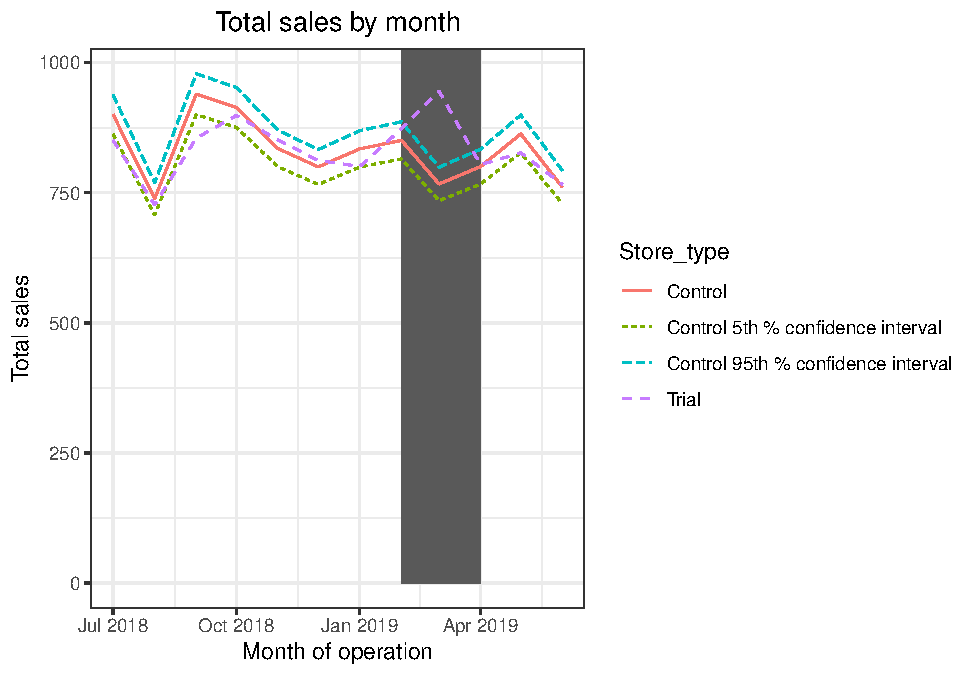
\includegraphics{InsideSherpa_Task2_files/figure-latex/unnamed-chunk-19-1}
The results show that the trial in store 86 is not significantly
different to its control store in the trial period as the trial store
performance lies inside the 5\% to 95\% confidence interval of the
control store in two of the three trial months. Let's have a look at
assessing this for the number of customers as well.

\begin{Shaded}
\begin{Highlighting}[]
\DocumentationTok{\#\#\#\# This would be a repeat of the steps before for total sales}
\DocumentationTok{\#\#\#\# Scale pre{-}trial control customers to match pre{-}trial trial store customers}
\NormalTok{scalingFactorForControlCust }\OtherTok{\textless{}{-}}\NormalTok{ preTrialMeasures[STORE\_NBR }\SpecialCharTok{==}\NormalTok{ trial\_store }\SpecialCharTok{\&}
\NormalTok{YEARMONTH }\SpecialCharTok{\textless{}} \DecValTok{201902}\NormalTok{, }\FunctionTok{sum}\NormalTok{(nCustomers)]}\SpecialCharTok{/}\NormalTok{preTrialMeasures[STORE\_NBR }\SpecialCharTok{==}\NormalTok{ control\_store }\SpecialCharTok{\&}
\NormalTok{YEARMONTH }\SpecialCharTok{\textless{}} \DecValTok{201902}\NormalTok{, }\FunctionTok{sum}\NormalTok{(nCustomers)]}
\DocumentationTok{\#\#\#\# Apply the scaling factor}
\NormalTok{measureOverTimeCusts }\OtherTok{\textless{}{-}}\NormalTok{ measureOverTime}
\NormalTok{scaledControlCustomers }\OtherTok{\textless{}{-}}\NormalTok{ measureOverTimeCusts[STORE\_NBR }\SpecialCharTok{==}\NormalTok{ control\_store,}
\NormalTok{                                            ][ , controlCustomers }\SpecialCharTok{:=}\NormalTok{ nCustomers}
\SpecialCharTok{*}\NormalTok{ scalingFactorForControlCust}
\NormalTok{                                            ][, Store\_type }\SpecialCharTok{:=} \FunctionTok{ifelse}\NormalTok{(STORE\_NBR}
\SpecialCharTok{==}\NormalTok{ trial\_store, }\StringTok{"Trial"}\NormalTok{,}
                                      \FunctionTok{ifelse}\NormalTok{(STORE\_NBR }\SpecialCharTok{==}\NormalTok{ control\_store,}
\StringTok{"Control"}\NormalTok{, }\StringTok{"Other stores"}\NormalTok{))}
\NormalTok{]}
\DocumentationTok{\#\#\#\# Calculate the percentage difference between scaled control sales and trial sales}
\NormalTok{percentageDiff }\OtherTok{\textless{}{-}} \FunctionTok{merge}\NormalTok{(scaledControlCustomers[, }\FunctionTok{c}\NormalTok{(}\StringTok{"YEARMONTH"}\NormalTok{,}
\StringTok{"controlCustomers"}\NormalTok{)],}
\NormalTok{                        measureOverTime[STORE\_NBR }\SpecialCharTok{==}\NormalTok{ trial\_store, }\FunctionTok{c}\NormalTok{(}\StringTok{"nCustomers"}\NormalTok{,}
\StringTok{"YEARMONTH"}\NormalTok{)],}
                        \AttributeTok{by =} \StringTok{"YEARMONTH"}
\NormalTok{                        )[, percentageDiff }\SpecialCharTok{:=}
\FunctionTok{abs}\NormalTok{(controlCustomers}\SpecialCharTok{{-}}\NormalTok{nCustomers)}\SpecialCharTok{/}\NormalTok{controlCustomers]}
\DocumentationTok{\#\#\#\# As our null hypothesis is that the trial period is the same as the pre{-}trial }
\DocumentationTok{\#\#\#\# period, let\textquotesingle{}s take the standard deviation based on the scaled percentage difference}
\DocumentationTok{\#\#\#\# in the pre{-}trial period}
\NormalTok{stdDev }\OtherTok{\textless{}{-}} \FunctionTok{sd}\NormalTok{(percentageDiff[YEARMONTH }\SpecialCharTok{\textless{}} \DecValTok{201902}\NormalTok{ , percentageDiff])}
\NormalTok{degreesOfFreedom }\OtherTok{\textless{}{-}} \DecValTok{7}
\DocumentationTok{\#\#\#\# Trial and control store number of customers}
\NormalTok{pastCustomers }\OtherTok{\textless{}{-}}\NormalTok{ measureOverTimeCusts[, nCusts }\SpecialCharTok{:=} \FunctionTok{mean}\NormalTok{(nCustomers), by }\OtherTok{=}
\FunctionTok{c}\NormalTok{(}\StringTok{"YEARMONTH"}\NormalTok{, }\StringTok{"Store\_type"}\NormalTok{)}
\NormalTok{                              ][Store\_type }\SpecialCharTok{\%in\%} \FunctionTok{c}\NormalTok{(}\StringTok{"Trial"}\NormalTok{, }\StringTok{"Control"}\NormalTok{), ]}
\DocumentationTok{\#\#\#\# Control store 95th percentile}
\NormalTok{pastCustomers\_Controls95 }\OtherTok{\textless{}{-}}\NormalTok{ pastCustomers[Store\_type }\SpecialCharTok{==} \StringTok{"Control"}\NormalTok{,}
\NormalTok{                                ][, nCusts }\SpecialCharTok{:=}\NormalTok{ nCusts }\SpecialCharTok{*}\NormalTok{ (}\DecValTok{1} \SpecialCharTok{+}\NormalTok{ stdDev }\SpecialCharTok{*} \DecValTok{2}\NormalTok{)}
\NormalTok{                                ][, Store\_type }\SpecialCharTok{:=} \StringTok{"Control 95th \% confidence}
\StringTok{interval"}\NormalTok{]}
\DocumentationTok{\#\#\#\# Control store 5th percentile}
\NormalTok{pastCustomers\_Controls5 }\OtherTok{\textless{}{-}}\NormalTok{ pastCustomers[Store\_type }\SpecialCharTok{==} \StringTok{"Control"}\NormalTok{,}
\NormalTok{                              ][, nCusts }\SpecialCharTok{:=}\NormalTok{ nCusts }\SpecialCharTok{*}\NormalTok{ (}\DecValTok{1} \SpecialCharTok{{-}}\NormalTok{ stdDev }\SpecialCharTok{*} \DecValTok{2}\NormalTok{)}
\NormalTok{                              ][, Store\_type }\SpecialCharTok{:=} \StringTok{"Control 5th \% confidence}
\StringTok{interval"}\NormalTok{]}
\NormalTok{trialAssessment }\OtherTok{\textless{}{-}} \FunctionTok{rbind}\NormalTok{(pastCustomers, pastCustomers\_Controls95,}
\NormalTok{pastCustomers\_Controls5)}
\DocumentationTok{\#\#\#\# Plotting these in one nice graph}
\FunctionTok{ggplot}\NormalTok{(trialAssessment, }\FunctionTok{aes}\NormalTok{(TransactionMonth, nCusts, }\AttributeTok{color =}\NormalTok{ Store\_type)) }\SpecialCharTok{+}
  \FunctionTok{geom\_rect}\NormalTok{(}\AttributeTok{data =}\NormalTok{ trialAssessment[ YEARMONTH }\SpecialCharTok{\textless{}} \DecValTok{201905} \SpecialCharTok{\&}\NormalTok{ YEARMONTH }\SpecialCharTok{\textgreater{}} \DecValTok{201901}\NormalTok{ ,],}
\FunctionTok{aes}\NormalTok{(}\AttributeTok{xmin =} \FunctionTok{min}\NormalTok{(TransactionMonth), }\AttributeTok{xmax =} \FunctionTok{max}\NormalTok{(TransactionMonth), }\AttributeTok{ymin =} \DecValTok{0}\NormalTok{ , }\AttributeTok{ymax =}
\ConstantTok{Inf}\NormalTok{, }\AttributeTok{color =} \ConstantTok{NULL}\NormalTok{), }\AttributeTok{show.legend =} \ConstantTok{FALSE}\NormalTok{) }\SpecialCharTok{+}
  \FunctionTok{geom\_line}\NormalTok{() }\SpecialCharTok{+}
  \FunctionTok{labs}\NormalTok{(}\AttributeTok{x =} \StringTok{"Month of operation"}\NormalTok{, }\AttributeTok{y =} \StringTok{"Total number of customers"}\NormalTok{, }\AttributeTok{title =} \StringTok{"Total}
\StringTok{number of customers by month"}\NormalTok{)}
\end{Highlighting}
\end{Shaded}

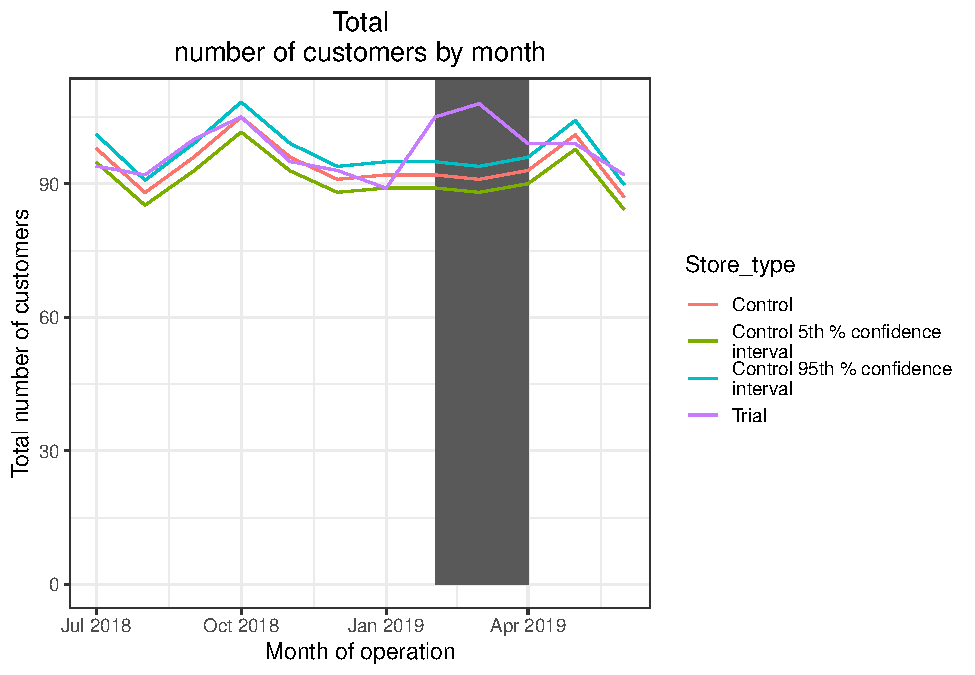
\includegraphics{InsideSherpa_Task2_files/figure-latex/unnamed-chunk-20-1}
It looks like the number of customers is significantly higher in all of
the three months. This seems to suggest that the trial had a significant
impact on increasing the number of customers in trial store 86 but as we
saw, sales were not significantly higher. We should check with the
Category Manager if there were special deals in the trial store that
were may have resulted in lower prices, impacting the results. \#\#
Trial store 88

\begin{Shaded}
\begin{Highlighting}[]
\DocumentationTok{\#\#\#\# Conduct the analysis on trial store 88.}
\NormalTok{measureOverTime }\OtherTok{\textless{}{-}}\NormalTok{ data[, .(}\AttributeTok{totSales =} \FunctionTok{sum}\NormalTok{(TOT\_SALES),}
\AttributeTok{nCustomers =} \FunctionTok{uniqueN}\NormalTok{(LYLTY\_CARD\_NBR),}
\AttributeTok{nTxnPerCust =} \FunctionTok{uniqueN}\NormalTok{(TXN\_ID)}\SpecialCharTok{/}\FunctionTok{uniqueN}\NormalTok{(LYLTY\_CARD\_NBR),}
\AttributeTok{nChipsPerTxn =} \FunctionTok{sum}\NormalTok{(PROD\_QTY)}\SpecialCharTok{/}\FunctionTok{uniqueN}\NormalTok{(TXN\_ID),}
\AttributeTok{avgPricePerUnit =} \FunctionTok{sum}\NormalTok{(TOT\_SALES)}\SpecialCharTok{/}\FunctionTok{sum}\NormalTok{(PROD\_QTY))}
\NormalTok{, by }\OtherTok{=} \FunctionTok{c}\NormalTok{(}\StringTok{"STORE\_NBR"}\NormalTok{, }\StringTok{"YEARMONTH"}\NormalTok{)][}\FunctionTok{order}\NormalTok{(STORE\_NBR, YEARMONTH)]}
\DocumentationTok{\#\#\#\# Use the functions from earlier to calculate the correlation of the sales and number of customers of each potential control store to the trial store}
\NormalTok{trial\_store }\OtherTok{\textless{}{-}} \DecValTok{88}
\NormalTok{corr\_nSales }\OtherTok{\textless{}{-}} \FunctionTok{calculateCorrelation}\NormalTok{(preTrialMeasures, }\FunctionTok{quote}\NormalTok{(totSales),trial\_store)}
\NormalTok{corr\_nCustomers }\OtherTok{\textless{}{-}} \FunctionTok{calculateCorrelation}\NormalTok{(preTrialMeasures, }\FunctionTok{quote}\NormalTok{(nCustomers), trial\_store)}
\DocumentationTok{\#\#\#\# Use the functions from earlier to calculate the magnitude distance of the sales and number of customers of each potential control store to the trial store}
\NormalTok{magnitude\_nSales }\OtherTok{\textless{}{-}} \FunctionTok{calculateMagnitudeDistance}\NormalTok{(preTrialMeasures, }\FunctionTok{quote}\NormalTok{(totSales), trial\_store)}
\NormalTok{magnitude\_nCustomers }\OtherTok{\textless{}{-}} \FunctionTok{calculateMagnitudeDistance}\NormalTok{(preTrialMeasures, }\FunctionTok{quote}\NormalTok{(nCustomers), trial\_store)}
\DocumentationTok{\#\#\#\# Create a combined score composed of correlation and magnitude by merging the correlations table and the magnitudes table, for each driver.}
\NormalTok{corr\_weight }\OtherTok{\textless{}{-}} \FloatTok{0.5}
\NormalTok{score\_nSales }\OtherTok{\textless{}{-}} \FunctionTok{merge}\NormalTok{(corr\_nSales, magnitude\_nSales, }\AttributeTok{by =} \FunctionTok{c}\NormalTok{(}\StringTok{"Store1"}\NormalTok{, }\StringTok{"Store2"}\NormalTok{))[ , scoreNSales }\SpecialCharTok{:=}\NormalTok{ (corr\_measure }\SpecialCharTok{+}\NormalTok{ mag\_measure)}\SpecialCharTok{/}\DecValTok{2}\NormalTok{]}
\NormalTok{score\_nCustomers }\OtherTok{\textless{}{-}} \FunctionTok{merge}\NormalTok{(corr\_nCustomers, magnitude\_nCustomers, }\AttributeTok{by =} \FunctionTok{c}\NormalTok{(}\StringTok{"Store1"}\NormalTok{, }\StringTok{"Store2"}\NormalTok{))[ , scoreNCust }\SpecialCharTok{:=}\NormalTok{ (corr\_measure }\SpecialCharTok{+}\NormalTok{ mag\_measure)}\SpecialCharTok{/}\DecValTok{2}\NormalTok{]}

\DocumentationTok{\#\#\#\# Combine scores across the drivers by merging sales scores and customer scores, and compute a final combined score.}
\NormalTok{score\_Control }\OtherTok{\textless{}{-}} \FunctionTok{merge}\NormalTok{(score\_nSales, score\_nCustomers, }\AttributeTok{by =} \FunctionTok{c}\NormalTok{(}\StringTok{"Store1"}\NormalTok{,}\StringTok{"Store2"}\NormalTok{))}
\NormalTok{score\_Control[, finalControlScore }\SpecialCharTok{:=}\NormalTok{ scoreNSales }\SpecialCharTok{*} \FloatTok{0.5} \SpecialCharTok{+}\NormalTok{ scoreNCust }\SpecialCharTok{*} \FloatTok{0.5}\NormalTok{]}
\DocumentationTok{\#\#\#\# Select control stores based on the highest matching store}
\DocumentationTok{\#\#\#\# (closest to 1 but not the store itself, i.e. the second ranked highest store)}
\DocumentationTok{\#\#\#\# Select control store for trial store 88}
\NormalTok{control\_store }\OtherTok{\textless{}{-}}\NormalTok{ score\_Control[Store1 }\SpecialCharTok{==}\NormalTok{ trial\_store, ][}\FunctionTok{order}\NormalTok{(}\SpecialCharTok{{-}}\NormalTok{finalControlScore)][}\DecValTok{2}\NormalTok{, Store2]}
\NormalTok{control\_store}
\end{Highlighting}
\end{Shaded}

\begin{verbatim}
## [1] 237
\end{verbatim}

We've now found store 237 to be a suitable control store for trial store
88. Again, let's check visually if the drivers are indeed similar in the
period before the trial. We'll look at total sales first.

\begin{Shaded}
\begin{Highlighting}[]
\DocumentationTok{\#\#\#\# Visual checks on trends based on the drivers}
\DocumentationTok{\#\#\#\# For the period before the trial, create a graph with total sales of the trial }
\DocumentationTok{\#\#\#\# store for each month, compared to the control store and other stores.}
\NormalTok{measureOverTimeSales }\OtherTok{\textless{}{-}}\NormalTok{ measureOverTime}
\NormalTok{pastSales }\OtherTok{\textless{}{-}}\NormalTok{ measureOverTimeSales[, Store\_type }\SpecialCharTok{:=} \FunctionTok{ifelse}\NormalTok{(STORE\_NBR }\SpecialCharTok{==}\NormalTok{ trial\_store, }\StringTok{"Trial"}\NormalTok{,}
\FunctionTok{ifelse}\NormalTok{(STORE\_NBR }\SpecialCharTok{==}\NormalTok{ control\_store, }\StringTok{"Control"}\NormalTok{, }\StringTok{"Other stores"}\NormalTok{))}
\NormalTok{][, totSales }\SpecialCharTok{:=} \FunctionTok{mean}\NormalTok{(totSales), by }\OtherTok{=} \FunctionTok{c}\NormalTok{(}\StringTok{"YEARMONTH"}\NormalTok{,}\StringTok{"Store\_type"}\NormalTok{)}
\NormalTok{][, TransactionMonth }\SpecialCharTok{:=} \FunctionTok{as.Date}\NormalTok{(}\FunctionTok{paste}\NormalTok{(YEARMONTH }\SpecialCharTok{\%/\%} \DecValTok{100}\NormalTok{, YEARMONTH }\SpecialCharTok{\%\%} \DecValTok{100}\NormalTok{, }\DecValTok{1}\NormalTok{, }\AttributeTok{sep =} \StringTok{"{-}"}\NormalTok{), }\StringTok{"\%Y{-}\%m{-}\%d"}\NormalTok{)}
\NormalTok{][YEARMONTH }\SpecialCharTok{\textless{}} \DecValTok{201903}\NormalTok{ , ]}
\FunctionTok{ggplot}\NormalTok{(pastSales, }\FunctionTok{aes}\NormalTok{(TransactionMonth, totSales, }\AttributeTok{color =}\NormalTok{ Store\_type)) }\SpecialCharTok{+}
\FunctionTok{geom\_line}\NormalTok{(}\FunctionTok{aes}\NormalTok{(}\AttributeTok{linetype =}\NormalTok{ Store\_type)) }\SpecialCharTok{+}
\FunctionTok{labs}\NormalTok{(}\AttributeTok{x =} \StringTok{"Month of operation"}\NormalTok{, }\AttributeTok{y =} \StringTok{"Total sales"}\NormalTok{, }\AttributeTok{title =} \StringTok{"Total sales by month"}\NormalTok{)}
\end{Highlighting}
\end{Shaded}

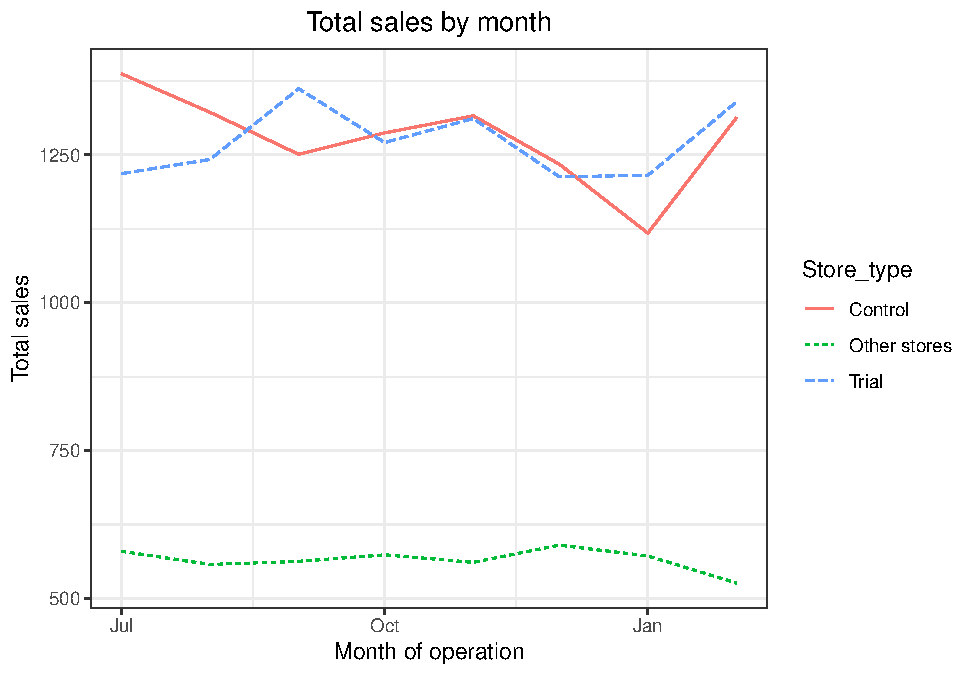
\includegraphics{InsideSherpa_Task2_files/figure-latex/unnamed-chunk-22-1.pdf}
Great, the trial and control stores have similar total sales. Next,
number of customers.

\begin{Shaded}
\begin{Highlighting}[]
\DocumentationTok{\#\#\#\# Visual checks on trends based on the drivers}
\DocumentationTok{\#\#\#\# For the period before the trial, create a graph with customer counts of the}
\DocumentationTok{\#\#\#\# trial store for each month, compared to the control store and other stores.}
\NormalTok{measureOverTimeCusts }\OtherTok{\textless{}{-}}\NormalTok{ measureOverTime}
\NormalTok{pastCustomers }\OtherTok{\textless{}{-}}\NormalTok{ measureOverTimeCusts[, Store\_type }\SpecialCharTok{:=} \FunctionTok{ifelse}\NormalTok{(STORE\_NBR }\SpecialCharTok{==}\NormalTok{ trial\_store, }\StringTok{"Trial"}\NormalTok{,}
\FunctionTok{ifelse}\NormalTok{(STORE\_NBR }\SpecialCharTok{==}\NormalTok{ control\_store, }\StringTok{"Control"}\NormalTok{, }\StringTok{"Other stores"}\NormalTok{))}
\NormalTok{][, numberCustomers }\SpecialCharTok{:=} \FunctionTok{mean}\NormalTok{(nCustomers), by }\OtherTok{=} \FunctionTok{c}\NormalTok{(}\StringTok{"YEARMONTH"}\NormalTok{, }\StringTok{"Store\_type"}\NormalTok{)}
\NormalTok{][, TransactionMonth }\SpecialCharTok{:=} \FunctionTok{as.Date}\NormalTok{(}\FunctionTok{paste}\NormalTok{(YEARMONTH }\SpecialCharTok{\%/\%}
                                        \DecValTok{100}\NormalTok{, YEARMONTH }\SpecialCharTok{\%\%} \DecValTok{100}\NormalTok{, }\DecValTok{1}\NormalTok{, }\AttributeTok{sep =} \StringTok{"{-}"}\NormalTok{), }\StringTok{"\%Y{-}\%m{-}\%d"}\NormalTok{)}
\NormalTok{][YEARMONTH }\SpecialCharTok{\textless{}} \DecValTok{201903}\NormalTok{ , ]}
\FunctionTok{ggplot}\NormalTok{(pastCustomers, }\FunctionTok{aes}\NormalTok{(TransactionMonth, numberCustomers, }\AttributeTok{color =}\NormalTok{ Store\_type)) }\SpecialCharTok{+} 
  \FunctionTok{geom\_line}\NormalTok{() }\SpecialCharTok{+} \FunctionTok{labs}\NormalTok{(}\AttributeTok{x =} \StringTok{"Month of operation"}\NormalTok{, }\AttributeTok{y =} \StringTok{"Total number of customers"}\NormalTok{, }\AttributeTok{title =} \StringTok{"Total number of customers by month"}\NormalTok{)}
\end{Highlighting}
\end{Shaded}

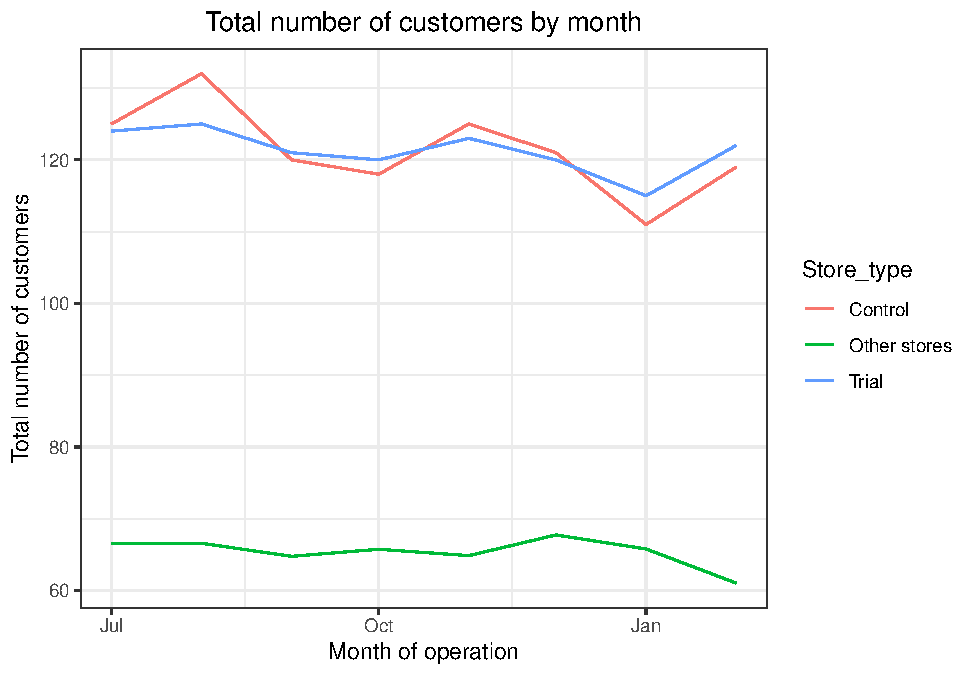
\includegraphics{InsideSherpa_Task2_files/figure-latex/unnamed-chunk-23-1.pdf}
Total number of customers of the control and trial stores are also
similar. Let's now assess the impact of the trial on sales.

\begin{Shaded}
\begin{Highlighting}[]
\DocumentationTok{\#\#\#\# Scale pre{-}trial control store sales to match pre{-}trial trial store sales}
\NormalTok{scalingFactorForControlSales }\OtherTok{\textless{}{-}}\NormalTok{ preTrialMeasures[STORE\_NBR }\SpecialCharTok{==}\NormalTok{ trial\_store }\SpecialCharTok{\&}
\NormalTok{YEARMONTH }\SpecialCharTok{\textless{}} \DecValTok{201902}\NormalTok{, }\FunctionTok{sum}\NormalTok{(totSales)]}\SpecialCharTok{/}\NormalTok{preTrialMeasures[STORE\_NBR }\SpecialCharTok{==}
\NormalTok{control\_store }\SpecialCharTok{\&}\NormalTok{ YEARMONTH }\SpecialCharTok{\textless{}} \DecValTok{201902}\NormalTok{, }\FunctionTok{sum}\NormalTok{(totSales)]}

\DocumentationTok{\#\#\#\# Apply the scaling factor}
\NormalTok{measureOverTimeSales }\OtherTok{\textless{}{-}}\NormalTok{ measureOverTime}
\NormalTok{scaledControlSales }\OtherTok{\textless{}{-}}\NormalTok{ measureOverTimeSales[STORE\_NBR }\SpecialCharTok{==}\NormalTok{ control\_store, ][ ,controlSales }\SpecialCharTok{:=}\NormalTok{ totSales }\SpecialCharTok{*}\NormalTok{ scalingFactorForControlSales]}

\DocumentationTok{\#\#\#\# Calculate the absolute percentage difference between scaled control sales and trial sales}
\NormalTok{percentageDiff }\OtherTok{\textless{}{-}} \FunctionTok{merge}\NormalTok{(scaledControlSales[, }\FunctionTok{c}\NormalTok{(}\StringTok{"YEARMONTH"}\NormalTok{, }\StringTok{"controlSales"}\NormalTok{)],measureOverTime[STORE\_NBR }\SpecialCharTok{==}\NormalTok{ trial\_store, }\FunctionTok{c}\NormalTok{(}\StringTok{"totSales"}\NormalTok{, }\StringTok{"YEARMONTH"}\NormalTok{)],}\AttributeTok{by =} \StringTok{"YEARMONTH"}\NormalTok{)[, percentageDiff }\SpecialCharTok{:=} \FunctionTok{abs}\NormalTok{(controlSales}\SpecialCharTok{{-}}\NormalTok{totSales)}\SpecialCharTok{/}\NormalTok{controlSales]}

\DocumentationTok{\#\#\#\# As our null hypothesis is that the trial period is the same as the pre{-}trial period, }
\DocumentationTok{\#\#\#\# let\textquotesingle{}s take the standard deviation based on the scaled percentage difference in the pre{-}trial period}
\NormalTok{stdDev }\OtherTok{\textless{}{-}} \FunctionTok{sd}\NormalTok{(percentageDiff[YEARMONTH }\SpecialCharTok{\textless{}} \DecValTok{201902}\NormalTok{ , percentageDiff])}
\NormalTok{degreesOfFreedom }\OtherTok{\textless{}{-}} \DecValTok{7}
\DocumentationTok{\#\#\#\# Trial and control store total sales}
\NormalTok{measureOverTimeSales }\OtherTok{\textless{}{-}}\NormalTok{ measureOverTime}
\NormalTok{pastSales }\OtherTok{\textless{}{-}}\NormalTok{ measureOverTimeSales[, Store\_type }\SpecialCharTok{:=} \FunctionTok{ifelse}\NormalTok{(STORE\_NBR }\SpecialCharTok{==}\NormalTok{ trial\_store, }\StringTok{"Trial"}\NormalTok{,}
\FunctionTok{ifelse}\NormalTok{(STORE\_NBR }\SpecialCharTok{==}\NormalTok{ control\_store, }\StringTok{"Control"}\NormalTok{, }\StringTok{"Other stores"}\NormalTok{))}
\NormalTok{][, totSales }\SpecialCharTok{:=} \FunctionTok{mean}\NormalTok{(totSales), by }\OtherTok{=} \FunctionTok{c}\NormalTok{(}\StringTok{"YEARMONTH"}\NormalTok{, }\StringTok{"Store\_type"}\NormalTok{)}
\NormalTok{][, TransactionMonth }\SpecialCharTok{:=} \FunctionTok{as.Date}\NormalTok{(}\FunctionTok{paste}\NormalTok{(YEARMONTH }\SpecialCharTok{\%/\%}\DecValTok{100}\NormalTok{, YEARMONTH }\SpecialCharTok{\%\%} \DecValTok{100}\NormalTok{, }\DecValTok{1}\NormalTok{, }\AttributeTok{sep =} \StringTok{"{-}"}\NormalTok{), }\StringTok{"\%Y{-}\%m{-}\%d"}\NormalTok{)}
\NormalTok{][Store\_type }\SpecialCharTok{\%in\%} \FunctionTok{c}\NormalTok{(}\StringTok{"Trial"}\NormalTok{, }\StringTok{"Control"}\NormalTok{), ]}
\DocumentationTok{\#\#\#\# Control store 95th percentile}
\NormalTok{pastSales\_Controls95 }\OtherTok{\textless{}{-}}\NormalTok{ pastSales[Store\_type }\SpecialCharTok{==} \StringTok{"Control"}\NormalTok{,}
\NormalTok{][, totSales }\SpecialCharTok{:=}\NormalTok{ totSales }\SpecialCharTok{*}\NormalTok{ (}\DecValTok{1} \SpecialCharTok{+}\NormalTok{ stdDev }\SpecialCharTok{*} \DecValTok{2}\NormalTok{)}
\NormalTok{][, Store\_type }\SpecialCharTok{:=} \StringTok{"Control 95th \% confidence interval"}\NormalTok{]}
\DocumentationTok{\#\#\#\# Control store 5th percentile}
\NormalTok{pastSales\_Controls5 }\OtherTok{\textless{}{-}}\NormalTok{ pastSales[Store\_type }\SpecialCharTok{==} \StringTok{"Control"}\NormalTok{,}
\NormalTok{][, totSales }\SpecialCharTok{:=}\NormalTok{ totSales }\SpecialCharTok{*}\NormalTok{ (}\DecValTok{1} \SpecialCharTok{{-}}\NormalTok{ stdDev }\SpecialCharTok{*} \DecValTok{2}\NormalTok{)}
\NormalTok{][, Store\_type }\SpecialCharTok{:=} \StringTok{"Control 5th \% confidence interval"}\NormalTok{]}
\NormalTok{trialAssessment }\OtherTok{\textless{}{-}} \FunctionTok{rbind}\NormalTok{(pastSales, pastSales\_Controls95, pastSales\_Controls5)}
\DocumentationTok{\#\#\#\# Plotting these in one nice graph}
\FunctionTok{ggplot}\NormalTok{(trialAssessment, }\FunctionTok{aes}\NormalTok{(TransactionMonth, totSales, }\AttributeTok{color =}\NormalTok{ Store\_type)) }\SpecialCharTok{+}
\FunctionTok{geom\_rect}\NormalTok{(}\AttributeTok{data =}\NormalTok{ trialAssessment[ YEARMONTH }\SpecialCharTok{\textless{}} \DecValTok{201905} \SpecialCharTok{\&}\NormalTok{ YEARMONTH }\SpecialCharTok{\textgreater{}} \DecValTok{201901}\NormalTok{ ,],}
\FunctionTok{aes}\NormalTok{(}\AttributeTok{xmin =} \FunctionTok{min}\NormalTok{(TransactionMonth), }\AttributeTok{xmax =} \FunctionTok{max}\NormalTok{(TransactionMonth), }\AttributeTok{ymin =} \DecValTok{0}\NormalTok{ ,}
\AttributeTok{ymax =} \ConstantTok{Inf}\NormalTok{, }\AttributeTok{color =} \ConstantTok{NULL}\NormalTok{), }\AttributeTok{show.legend =} \ConstantTok{FALSE}\NormalTok{) }\SpecialCharTok{+} 
  \FunctionTok{geom\_line}\NormalTok{(}\FunctionTok{aes}\NormalTok{(}\AttributeTok{linetype =}\NormalTok{ Store\_type)) }\SpecialCharTok{+} 
  \FunctionTok{labs}\NormalTok{(}\AttributeTok{x =} \StringTok{"Month of operation"}\NormalTok{, }\AttributeTok{y =} \StringTok{"Total sales"}\NormalTok{, }\AttributeTok{title =} \StringTok{"Total sales by month"}\NormalTok{)}
\end{Highlighting}
\end{Shaded}

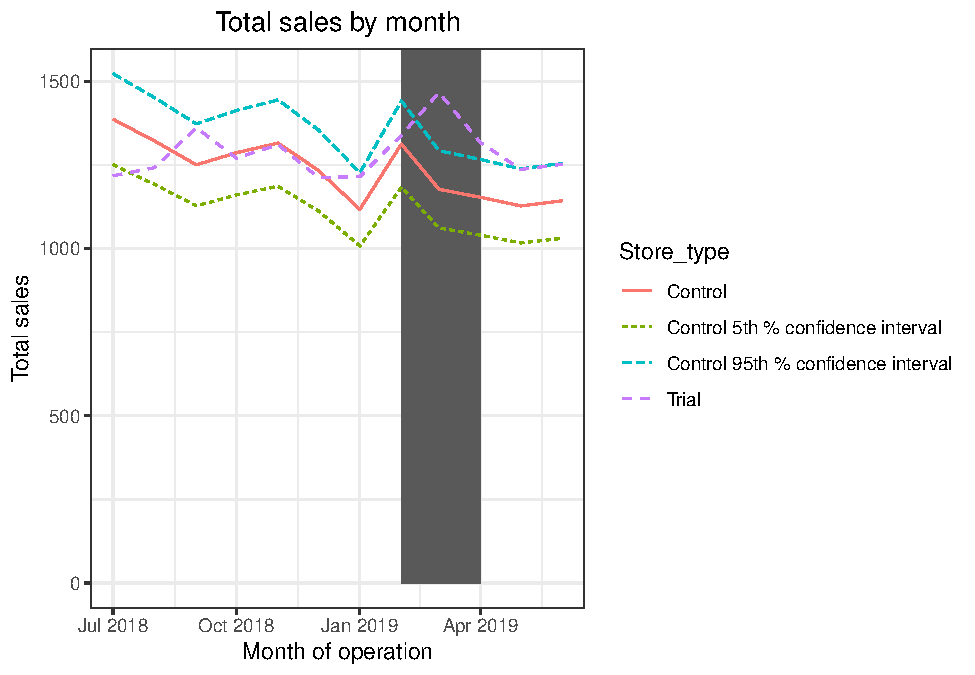
\includegraphics{InsideSherpa_Task2_files/figure-latex/unnamed-chunk-24-1}
The results show that the trial in store 88 is significantly different
to its control store in the trial period as the trial store performance
lies outside of the 5\% to 95\% confidence interval of the control store
in two of the three trial months. Let's have a look at assessing this
for number of customers as well.

\begin{Shaded}
\begin{Highlighting}[]
\DocumentationTok{\#\#\#\# This would be a repeat of the steps before for total sales}
\DocumentationTok{\#\#\#\# Scale pre{-}trial control store customers to match pre{-}trial trial store customers}
\NormalTok{scalingFactorForControlCust }\OtherTok{\textless{}{-}}\NormalTok{ preTrialMeasures[STORE\_NBR }\SpecialCharTok{==}\NormalTok{ trial\_store }\SpecialCharTok{\&}
\NormalTok{YEARMONTH }\SpecialCharTok{\textless{}} \DecValTok{201902}\NormalTok{, }\FunctionTok{sum}\NormalTok{(nCustomers)]}\SpecialCharTok{/}\NormalTok{preTrialMeasures[STORE\_NBR }\SpecialCharTok{==}
\NormalTok{control\_store }\SpecialCharTok{\&}\NormalTok{ YEARMONTH }\SpecialCharTok{\textless{}} \DecValTok{201902}\NormalTok{, }\FunctionTok{sum}\NormalTok{(nCustomers)]}

\DocumentationTok{\#\#\#\# Apply the scaling factor}
\NormalTok{measureOverTimeCusts }\OtherTok{\textless{}{-}}\NormalTok{ measureOverTime}
\NormalTok{scaledControlCustomers }\OtherTok{\textless{}{-}}\NormalTok{ measureOverTimeCusts[STORE\_NBR }\SpecialCharTok{==}\NormalTok{ control\_store,}
\NormalTok{][ , controlCustomers }\SpecialCharTok{:=}\NormalTok{ nCustomers }\SpecialCharTok{*}\NormalTok{ scalingFactorForControlCust}
\NormalTok{][, Store\_type }\SpecialCharTok{:=} \FunctionTok{ifelse}\NormalTok{(STORE\_NBR }\SpecialCharTok{==}\NormalTok{ trial\_store, }\StringTok{"Trial"}\NormalTok{,}
\FunctionTok{ifelse}\NormalTok{(STORE\_NBR }\SpecialCharTok{==}\NormalTok{ control\_store,}\StringTok{"Control"}\NormalTok{, }\StringTok{"Other stores"}\NormalTok{))}
\NormalTok{]}
\DocumentationTok{\#\#\#\# Calculate the absolute percentage difference between scaled control sales and trial sales}
\NormalTok{percentageDiff }\OtherTok{\textless{}{-}} \FunctionTok{merge}\NormalTok{(scaledControlCustomers[, }\FunctionTok{c}\NormalTok{(}\StringTok{"YEARMONTH"}\NormalTok{,}\StringTok{"controlCustomers"}\NormalTok{)],measureOverTime[STORE\_NBR }\SpecialCharTok{==}\NormalTok{ trial\_store, }\FunctionTok{c}\NormalTok{(}\StringTok{"nCustomers"}\NormalTok{, }\StringTok{"YEARMONTH"}\NormalTok{)],}
\AttributeTok{by =} \StringTok{"YEARMONTH"}\NormalTok{)[, percentageDiff }\SpecialCharTok{:=} \FunctionTok{abs}\NormalTok{(controlCustomers}\SpecialCharTok{{-}}\NormalTok{nCustomers)}\SpecialCharTok{/}\NormalTok{controlCustomers]}

\DocumentationTok{\#\#\#\# As our null hypothesis is that the trial period is the same as the pre{-}trial}
\DocumentationTok{\#\#\#\# period, let\textquotesingle{}s take the standard deviation based on the scaled percentage \#\#\#\# difference in the pre{-}trial period}

\NormalTok{stdDev }\OtherTok{\textless{}{-}} \FunctionTok{sd}\NormalTok{(percentageDiff[YEARMONTH }\SpecialCharTok{\textless{}} \DecValTok{201902}\NormalTok{ , percentageDiff])}
\NormalTok{degreesOfFreedom }\OtherTok{\textless{}{-}} \DecValTok{7} 
\CommentTok{\# note that there are 8 months in the pre{-}trial period hence 8 {-} 1 = 7 degrees of freedom}
\DocumentationTok{\#\#\#\# Trial and control store number of customers}
\NormalTok{pastCustomers }\OtherTok{\textless{}{-}}\NormalTok{ measureOverTimeCusts[, nCusts }\SpecialCharTok{:=} \FunctionTok{mean}\NormalTok{(nCustomers), by }\OtherTok{=} \FunctionTok{c}\NormalTok{(}\StringTok{"YEARMONTH"}\NormalTok{, }\StringTok{"Store\_type"}\NormalTok{)}
\NormalTok{][Store\_type }\SpecialCharTok{\%in\%} \FunctionTok{c}\NormalTok{(}\StringTok{"Trial"}\NormalTok{, }\StringTok{"Control"}\NormalTok{), ]}

\DocumentationTok{\#\#\#\# Control store 95th percentile}
\NormalTok{pastCustomers\_Controls95 }\OtherTok{\textless{}{-}}\NormalTok{ pastCustomers[Store\_type }\SpecialCharTok{==} \StringTok{"Control"}\NormalTok{,}
\NormalTok{][, nCusts }\SpecialCharTok{:=}\NormalTok{ nCusts }\SpecialCharTok{*}\NormalTok{ (}\DecValTok{1} \SpecialCharTok{+}\NormalTok{ stdDev }\SpecialCharTok{*} \DecValTok{2}\NormalTok{)}
\NormalTok{][, Store\_type }\SpecialCharTok{:=} \StringTok{"Control 95th \% confidence interval"}\NormalTok{]}
\DocumentationTok{\#\#\#\# Control store 5th percentile}
\NormalTok{pastCustomers\_Controls5 }\OtherTok{\textless{}{-}}\NormalTok{ pastCustomers[Store\_type }\SpecialCharTok{==} \StringTok{"Control"}\NormalTok{,}
\NormalTok{][, nCusts }\SpecialCharTok{:=}\NormalTok{ nCusts }\SpecialCharTok{*}\NormalTok{ (}\DecValTok{1} \SpecialCharTok{{-}}\NormalTok{ stdDev }\SpecialCharTok{*} \DecValTok{2}\NormalTok{)}
\NormalTok{][, Store\_type }\SpecialCharTok{:=} \StringTok{"Control 5th \% confidence interval"}\NormalTok{]}
\DocumentationTok{\#\#\#\# Combine the tables pastSales, pastSales\_Controls95, pastSales\_Controls5}
\NormalTok{trialAssessment }\OtherTok{\textless{}{-}} \FunctionTok{rbind}\NormalTok{(pastCustomers, pastCustomers\_Controls95,pastCustomers\_Controls5)}
\DocumentationTok{\#\#\#\# Plotting these in one nice graph}
\FunctionTok{ggplot}\NormalTok{(trialAssessment, }\FunctionTok{aes}\NormalTok{(TransactionMonth, nCusts, }\AttributeTok{color =}\NormalTok{ Store\_type)) }\SpecialCharTok{+}
  \FunctionTok{geom\_rect}\NormalTok{(}\AttributeTok{data =}\NormalTok{ trialAssessment[ YEARMONTH }\SpecialCharTok{\textless{}} \DecValTok{201905} \SpecialCharTok{\&}\NormalTok{ YEARMONTH }\SpecialCharTok{\textgreater{}} \DecValTok{201901}\NormalTok{ ,],}
\FunctionTok{aes}\NormalTok{(}\AttributeTok{xmin =} \FunctionTok{min}\NormalTok{(TransactionMonth), }\AttributeTok{xmax =} \FunctionTok{max}\NormalTok{(TransactionMonth), }\AttributeTok{ymin =} \DecValTok{0}\NormalTok{ ,}
\AttributeTok{ymax =} \ConstantTok{Inf}\NormalTok{, }\AttributeTok{color =} \ConstantTok{NULL}\NormalTok{), }\AttributeTok{show.legend =} \ConstantTok{FALSE}\NormalTok{) }\SpecialCharTok{+} \FunctionTok{geom\_line}\NormalTok{() }\SpecialCharTok{+} 
\FunctionTok{labs}\NormalTok{(}\AttributeTok{x =} \StringTok{"Month of operation"}\NormalTok{, }\AttributeTok{y =} \StringTok{"Total number of customers"}\NormalTok{, }\AttributeTok{title =} \StringTok{"Total number of customers by month"}\NormalTok{)}
\end{Highlighting}
\end{Shaded}

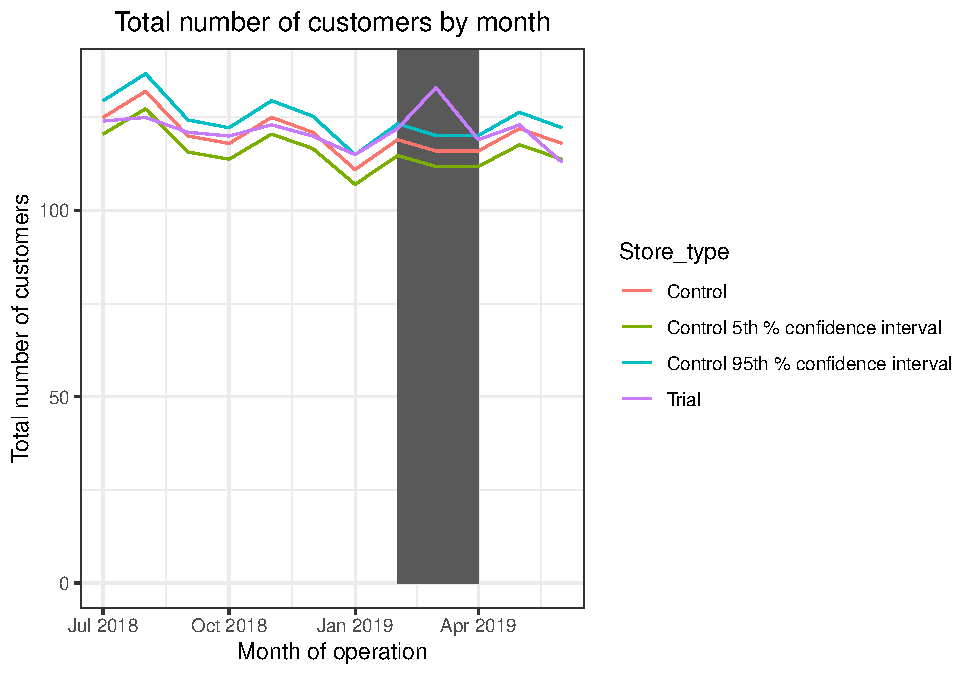
\includegraphics{InsideSherpa_Task2_files/figure-latex/unnamed-chunk-25-1}
Total number of customers in the trial period for the trial store is
significantly higher than the control store for two out of three months,
which indicates a positive trial effect. \#\# Conclusion Good work!
We've found control stores 233, 155, 237 for trial stores 77, 86 and 88
respectively. The results for trial stores 77 and 88 during the trial
period show a significant difference in at least two of the three trial
months but this is not the case for trial store 86. We can check with
the client if the implementation of the trial was different in trial
store 86 but overall, the trial shows a significant increase in sales.
Now that we have finished our analysis, we can prepare our presentation
to the Category Manager.

\end{document}
